% !TEX root = ../report.tex
\section*{The Experiments} \label{sec:experiments}
\addcontentsline{toc}{section}{The Experiments}
In this section we will discuss some elements of the experiment setup in greater detail, improvements to the experiment and compare the procedures from this and last semester.

\subsection*{Improvements to the system}\label{sec:systemImprovements}
\addcontentsline{toc}{subsection}{Improvements to the system}
We made some improvements to the system, compared to last semester, by using the newer Kinect for tracking bodies and detecting hands.

\subsection*{Improvements of the demo videos}\label{sec:videoslastsemester}
\addcontentsline{toc}{subsection}{Improvements of the demo videos}
When we did the experiment last semester we also had demonstration videos for the participants to look at if they were in doubt of how to perform a certain technique.
The way we did it then was to have the videos run in a loop on the small screen while the test started on the big screen.
Participants were able to start the test even after just seeing the title of the technique they were suppose to do and last semester we saw people jumping straight into it without having looked at the videos of the techniques. 
When this would happen they would simply spend more time in the beginning trying to figure the technique out for themselves.
If they were not successful performing the technique they would finally turn their attention to the demonstration of the technique.
During the experiment some participants noted that they did not notice the video of the technique running in a loop on the small screen.

The quality of the videos we used last semester were not good and people often complained that they were not clear and that they could not clearly see who the technique should be performed.
The videos were shot from two different perspectives and the phone appeared very small on the screen and was not easy to see.
The tempo of the videos and the cuts to white text on black background made the video seem unconnected and possibly a little hard to follow.\\

For this semester we changed the procedure for how we introduced the participants to the techniques and we also changed all the demonstration videos.
The procedure was changed such that participants had to watch the technique being performed two times before the test would start and they could start using the technique themselves.
Another change we made to the procedure were to have the video play on the large screen initially and after two iterations on the large screen the video played in a loop on the small screen.
The videos were changed so they are easier to understand and visibly more clear than were the case previously for example with the interaction on the phone being hard to see.
In the new videos a technique is explained in a slower pace and without cuts to a black screen with white text and we zoomed in on the phone as can be seen in \Cref{fig:demovideC}.
Four screenshots of the Push Throw technique demo video is shown in \Cref{fig:demovideo}.

\begin{figure}[H]
\subfloat[]{\includegraphics[width = 0.5\columnwidth]{images/demovideo1.pdf}\label{fig:demovideA}}
\subfloat[]{\includegraphics[width = 0.5\columnwidth]{images/demovideo2.pdf}\label{fig:demovideB}}\\
\subfloat[]{\includegraphics[width = 0.5\columnwidth]{images/demovideo3.pdf}\label{fig:demovideC}}
\subfloat[]{\includegraphics[width = 0.5\columnwidth]{images/demovideo4.pdf}\label{fig:demovideD}}
\caption{The images here shows the screen at different times during the demonstration video. The video was shown to the participant before each technique test starts. In \protect\subref{fig:demovideA} the technique is being presented with the direction and the name of the technique. In \protect\subref{fig:demovideB}, \protect\subref{fig:demovideC}, and \protect\subref{fig:demovideD} the video pauses and the participant will be able to read the instructions on the screen.}
\label{fig:demovideo}
\end{figure}

% !TEX root = ../report.tex
\section*{Techniques}\label{sec:techniques}
\addcontentsline{toc}{section}{Techniques}

\begin{figure}[H]
	\subfloat[]{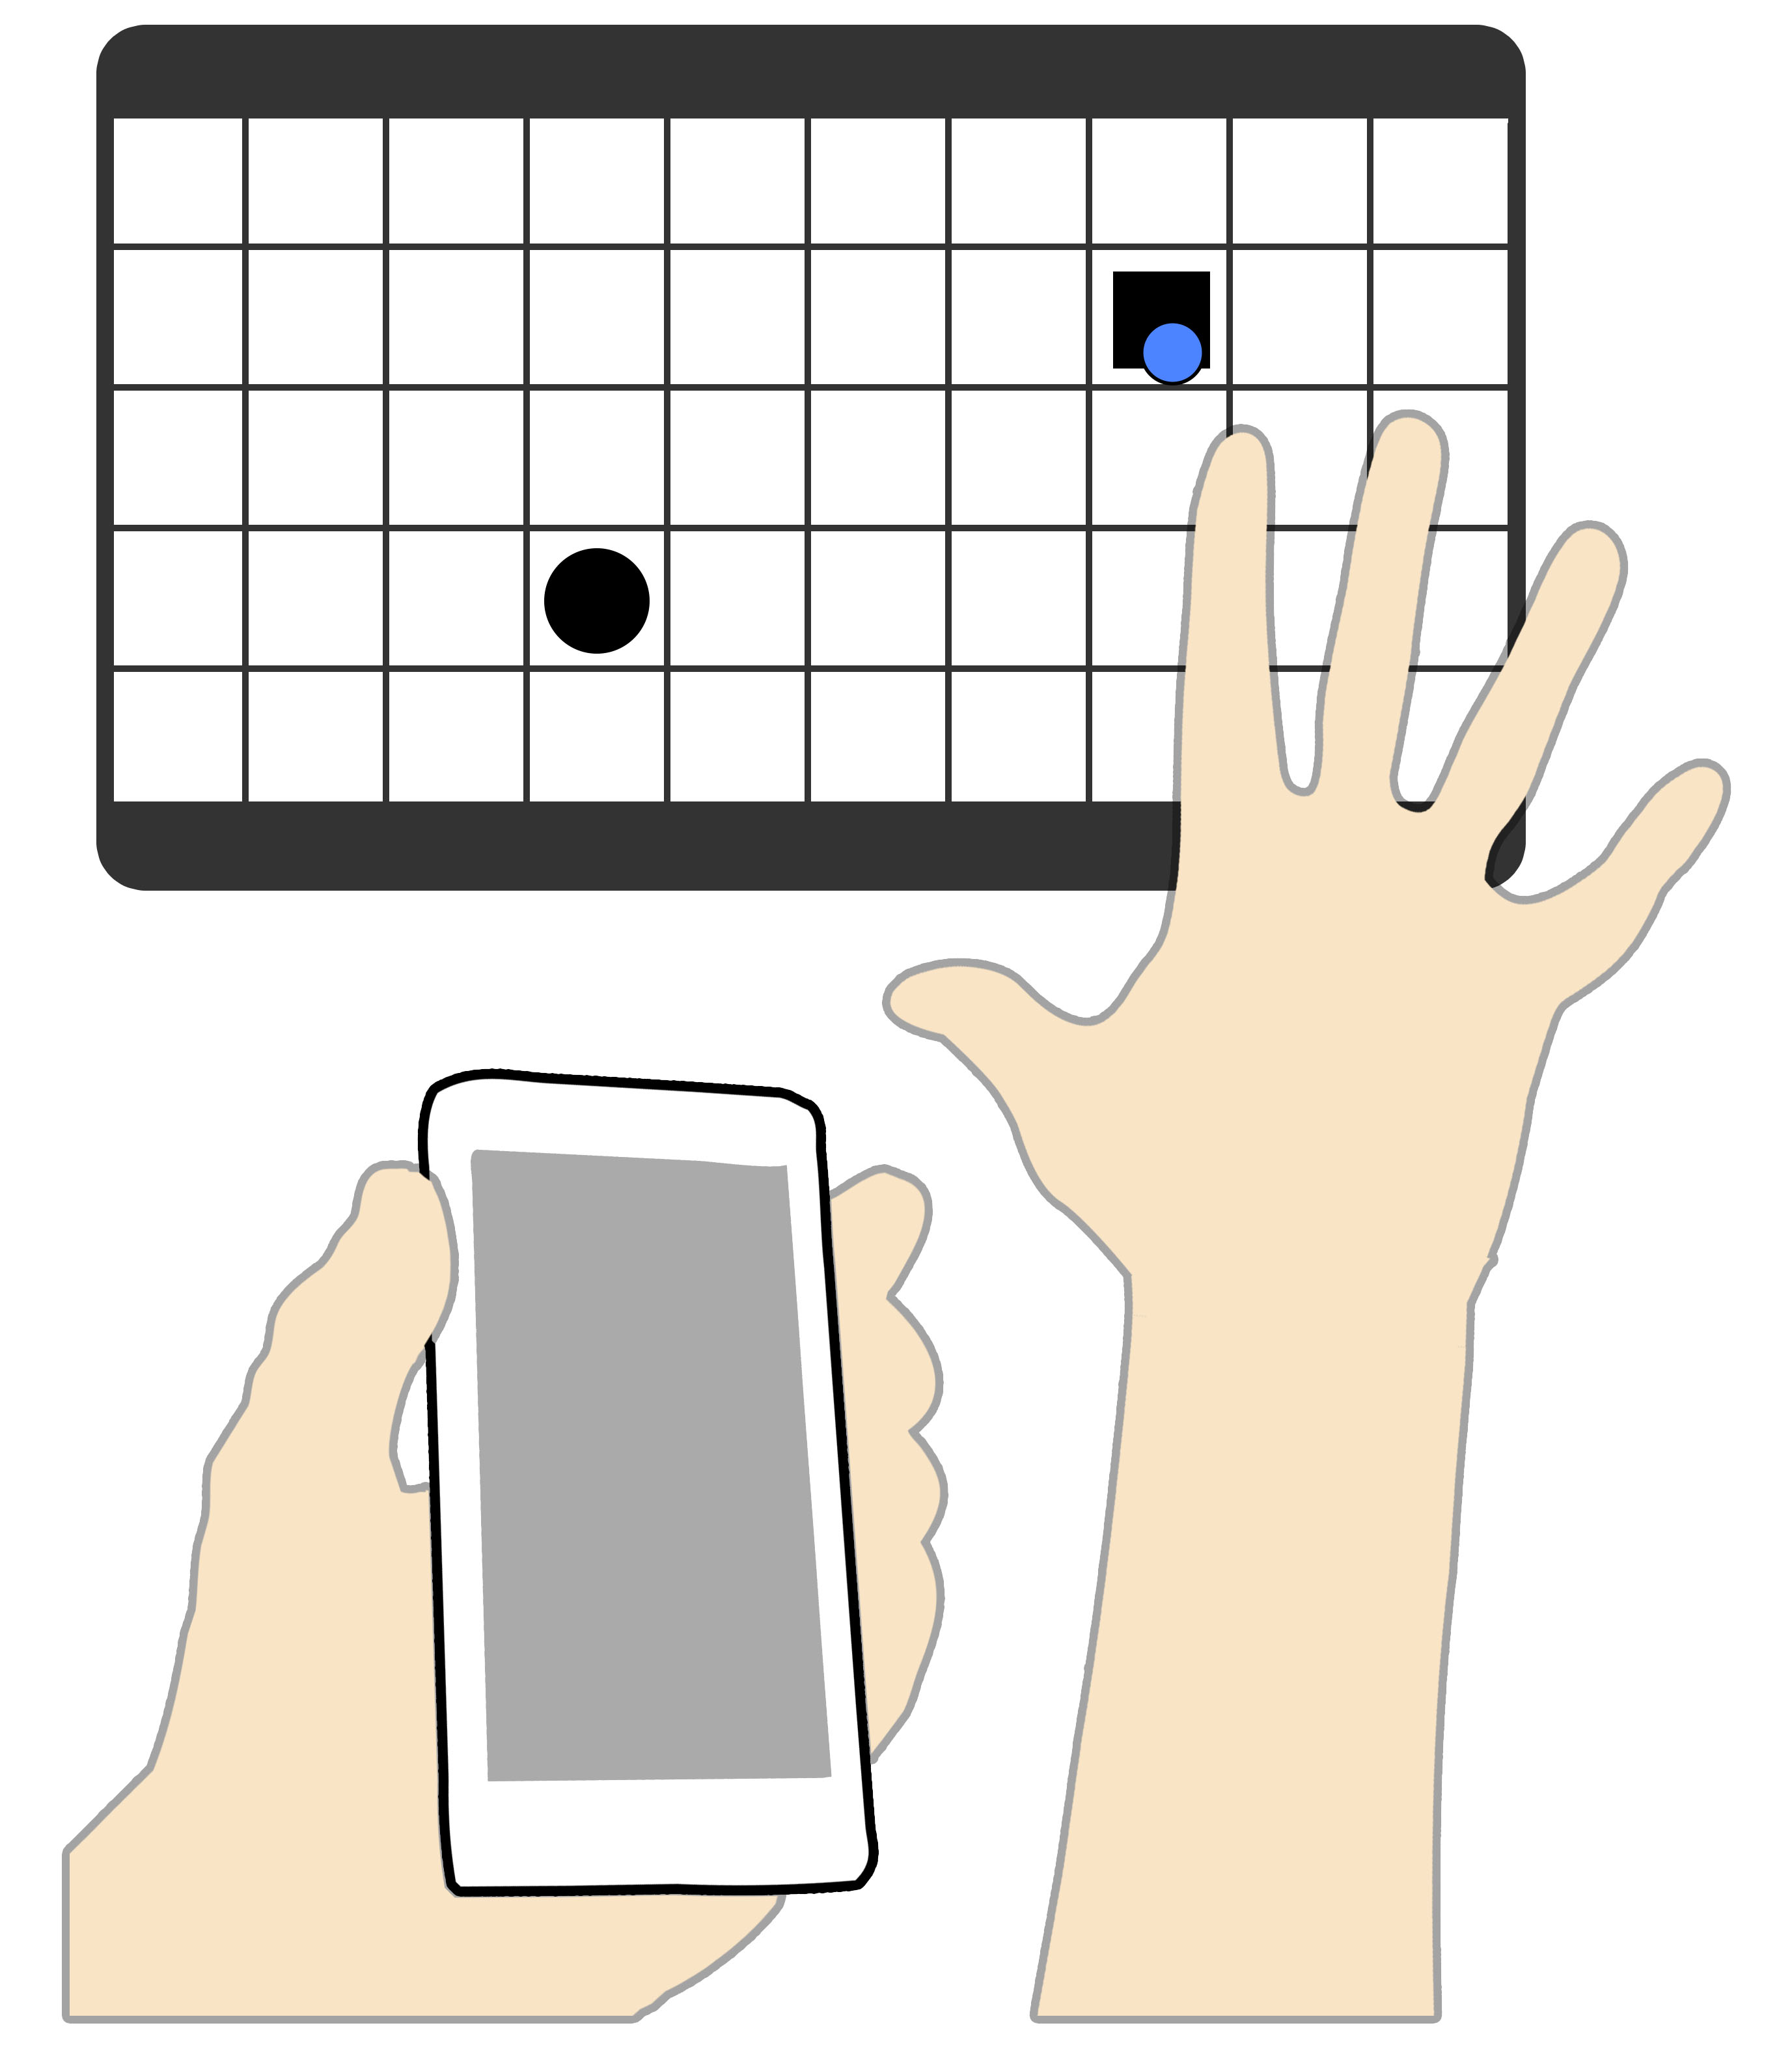
\includegraphics[width = 0.33\columnwidth]{images/techniques/grabPull1.jpg}\label{fig:grabPull1}}
	\subfloat[]{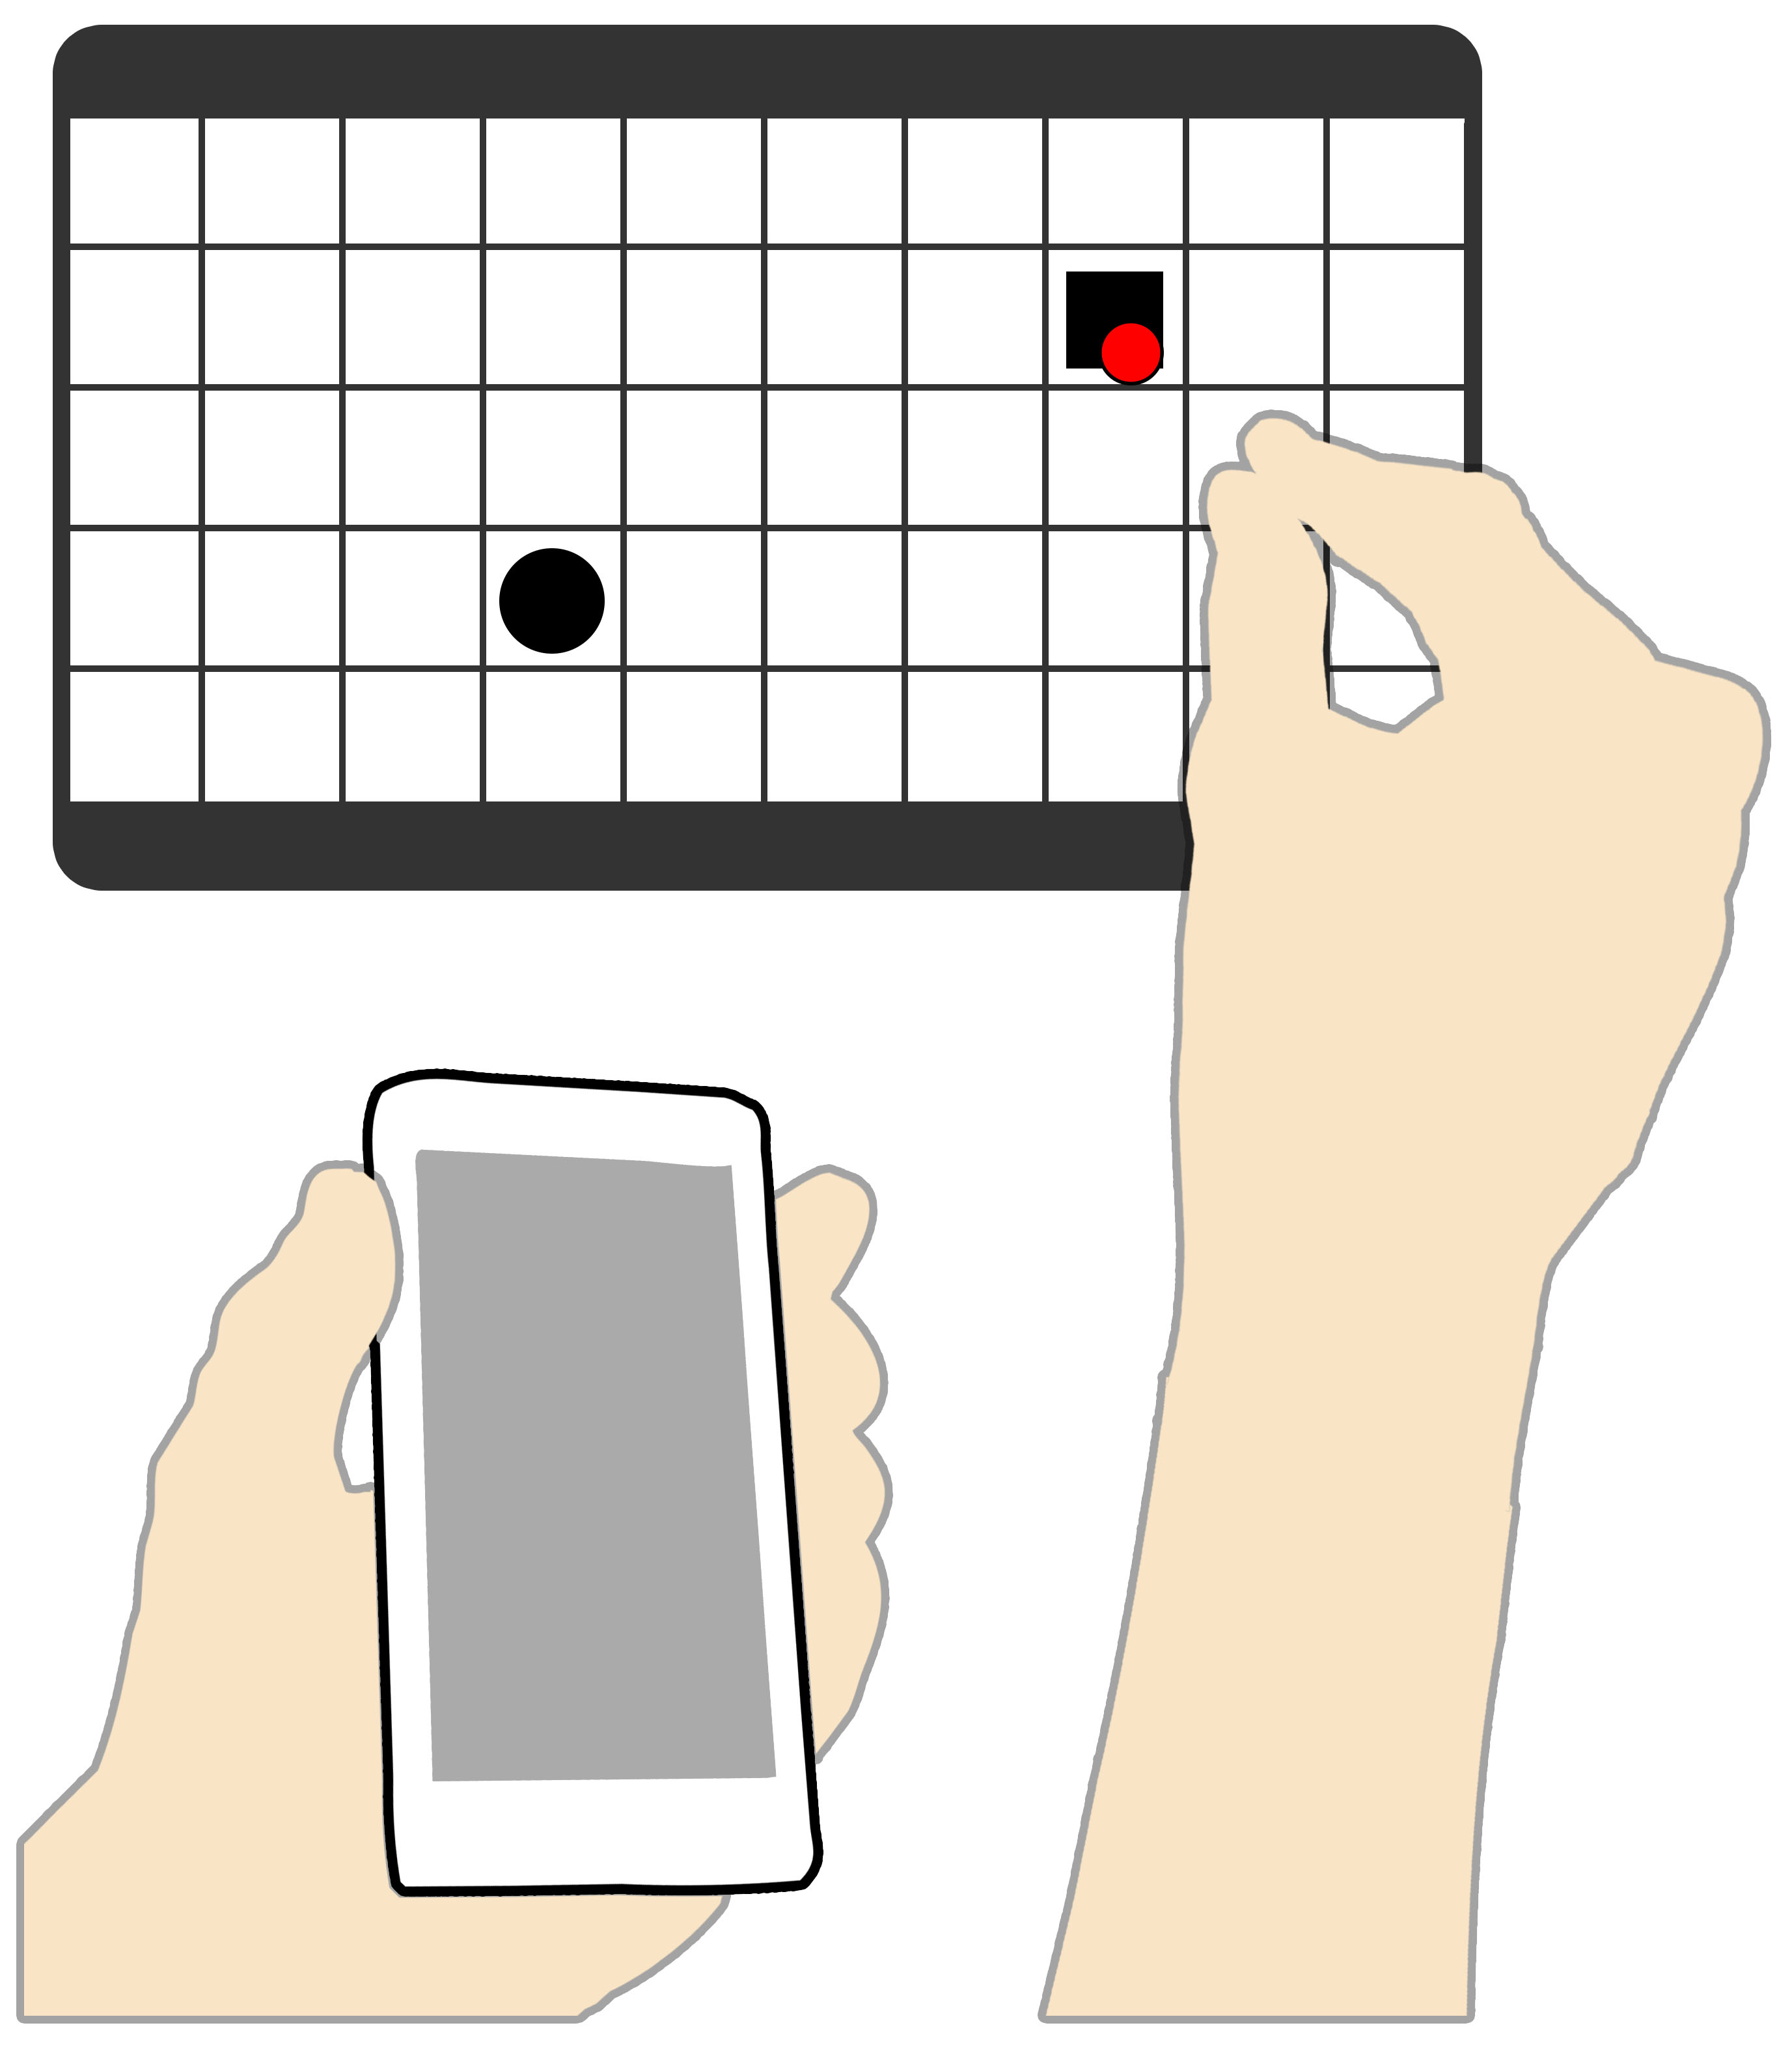
\includegraphics[width = 0.33\columnwidth]{images/techniques/grabPull2.jpg}\label{fig:grabPull2}}
	\subfloat[]{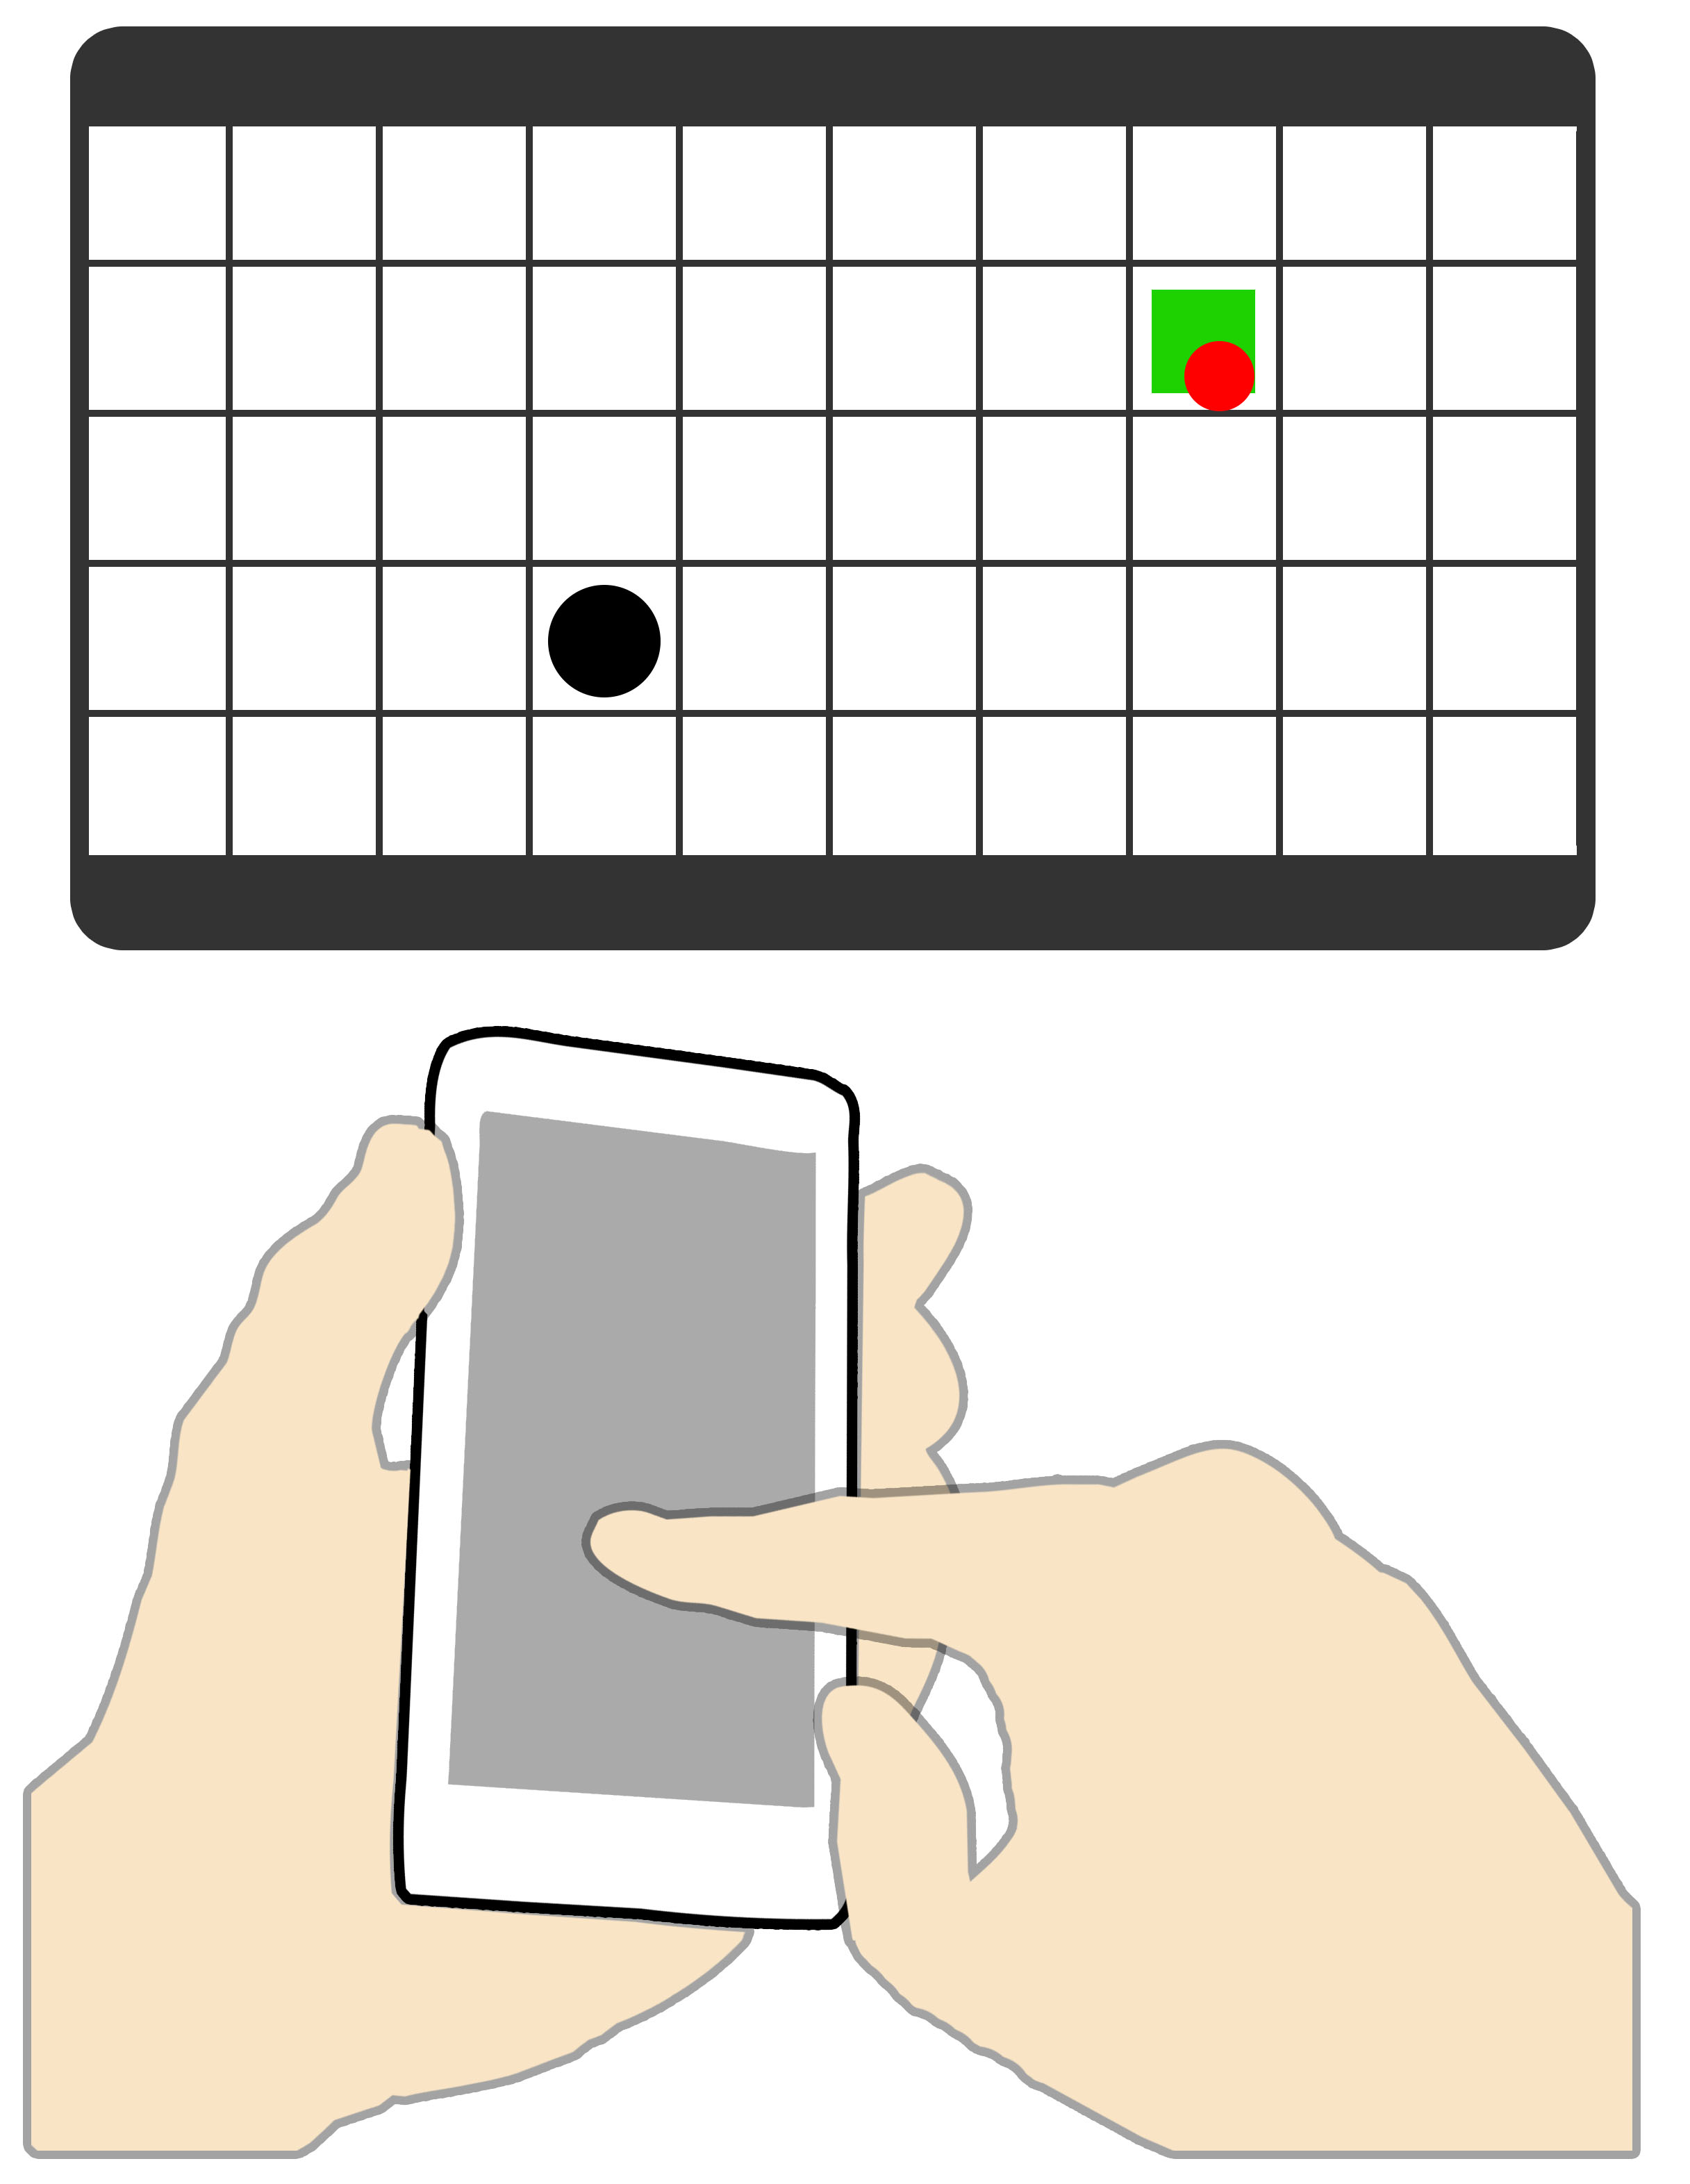
\includegraphics[width = 0.33\columnwidth]{images/techniques/grabPull3.jpg}\label{fig:grabPull3}}
	\caption{\push \grab technique}
	\label{fig:grabTechnique}
\end{figure}

\begin{figure}[H]
	\subfloat[]{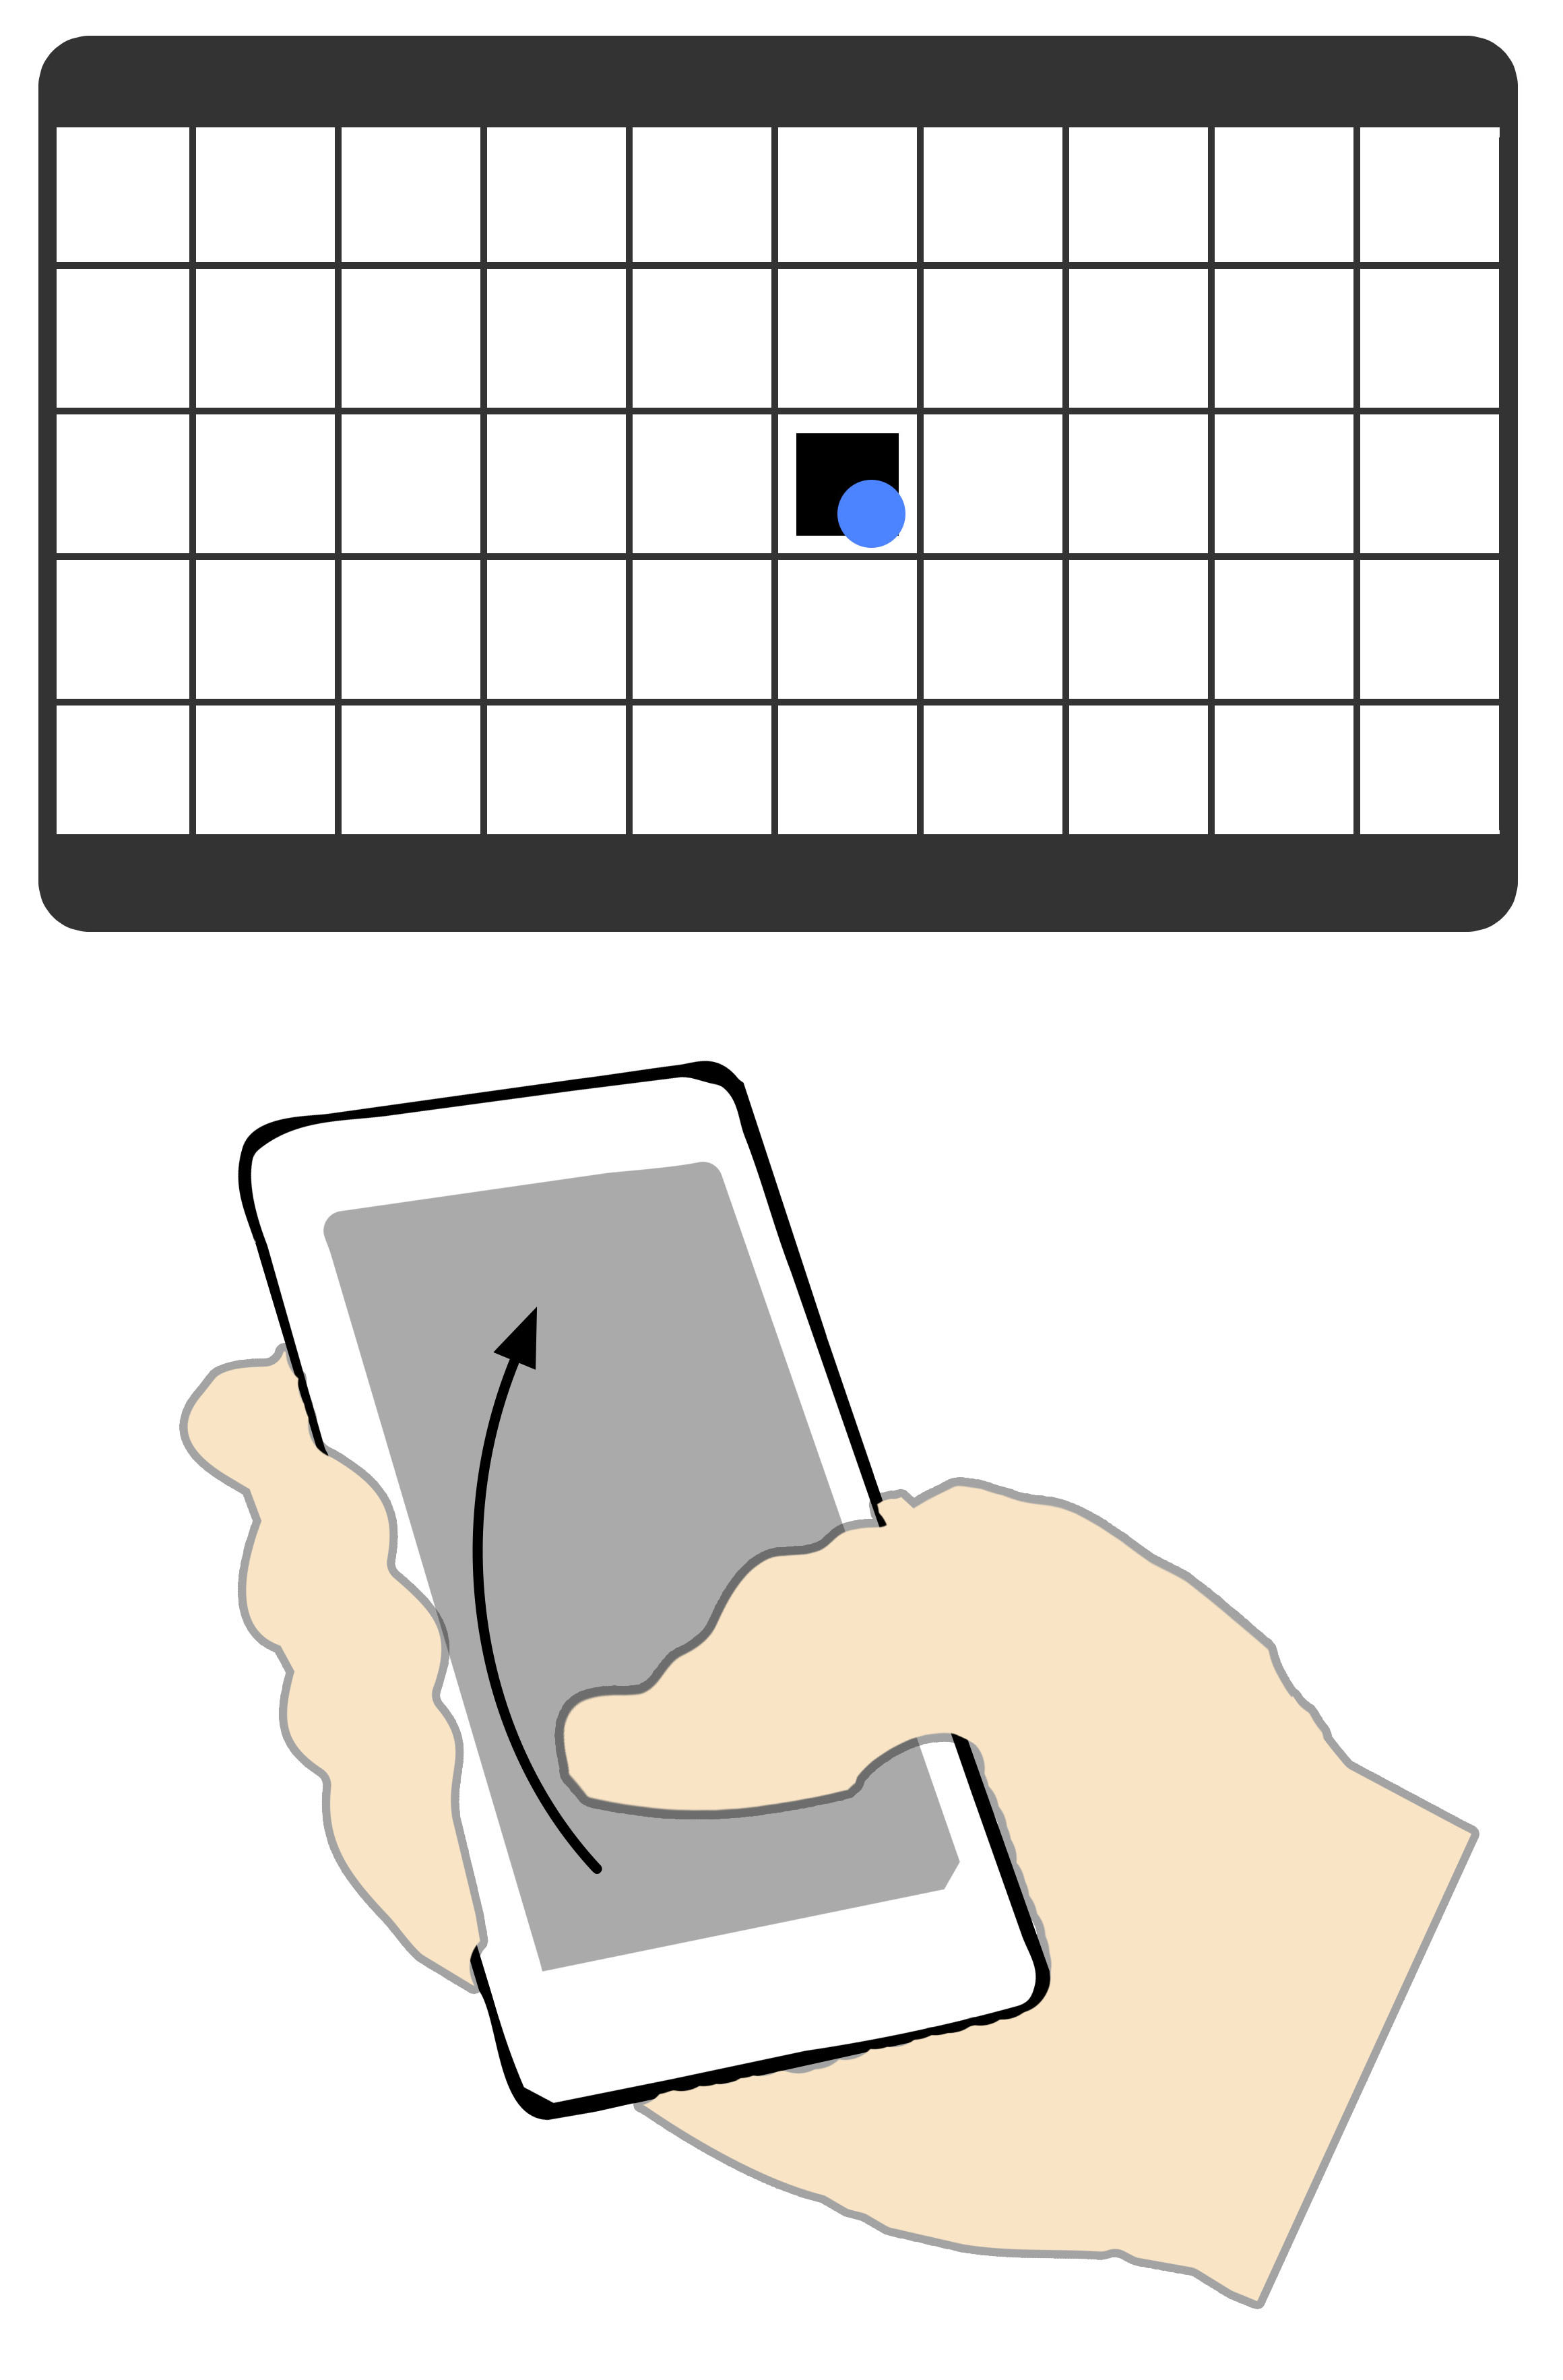
\includegraphics[width = 0.33\columnwidth]{images/techniques/swipePush1.jpg}\label{fig:swipePush1}}
	\subfloat[]{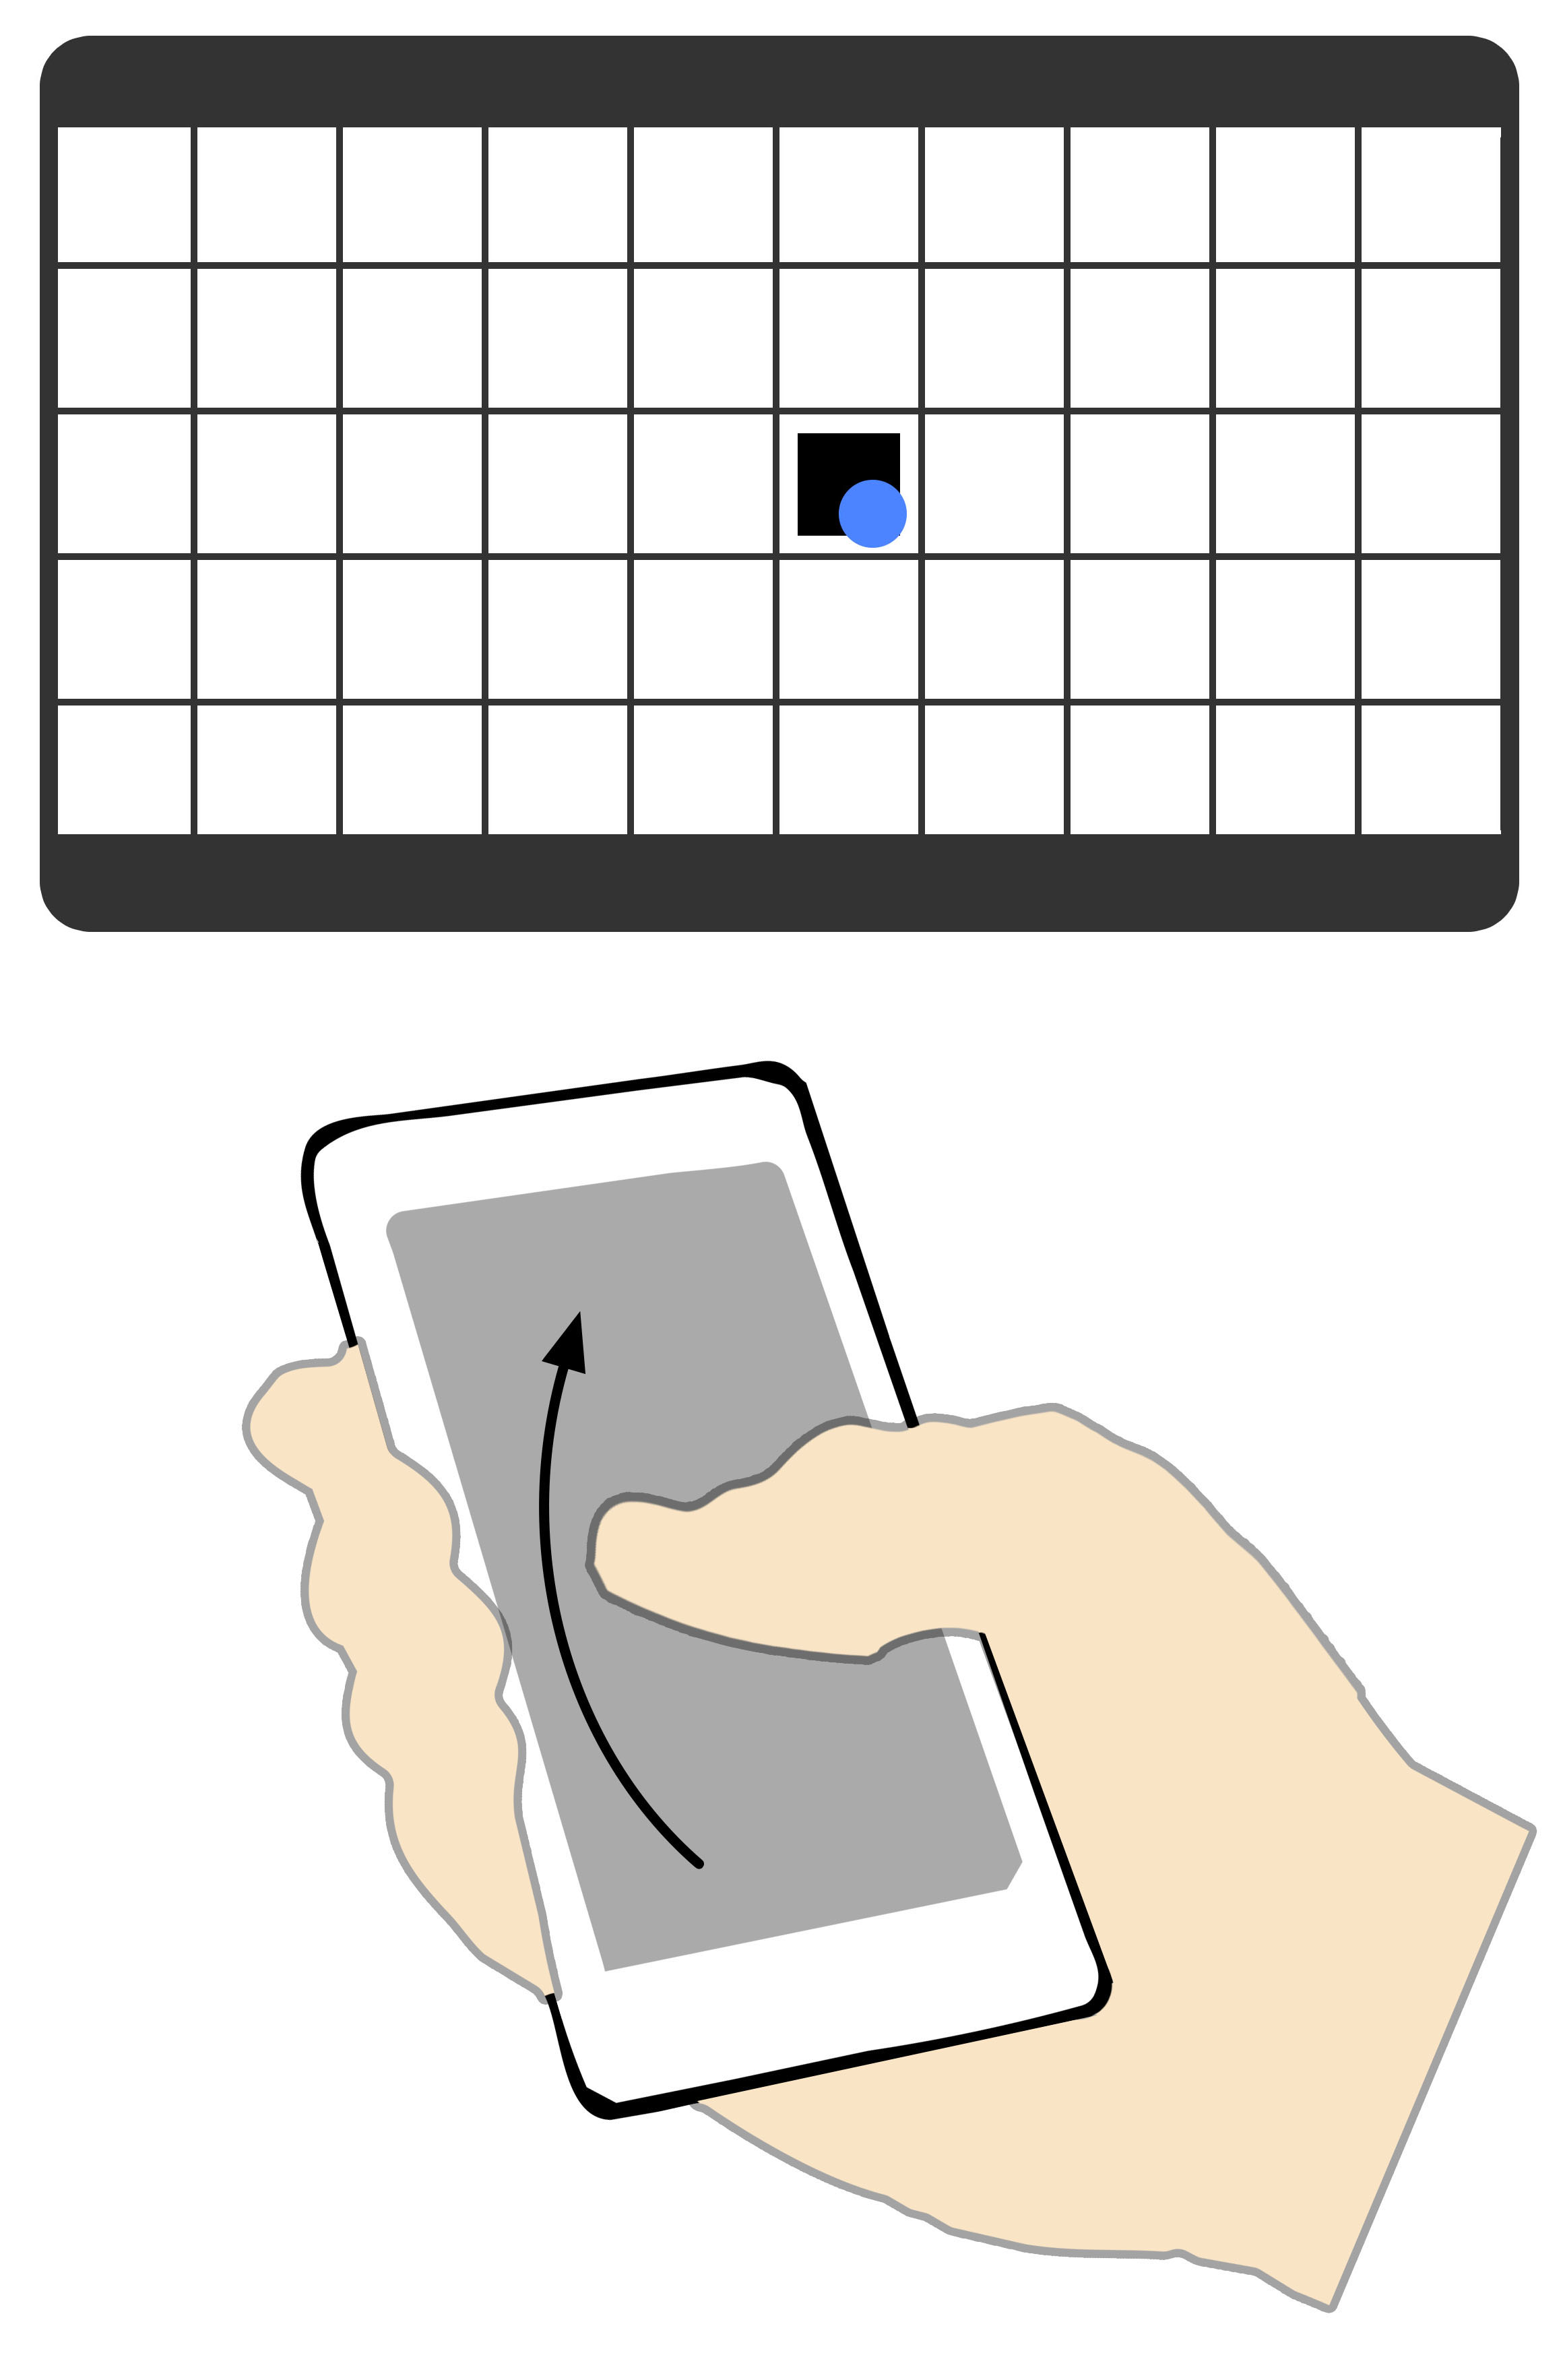
\includegraphics[width = 0.33\columnwidth]{images/techniques/swipePush2.jpg}\label{fig:swipePush2}}
	\subfloat[]{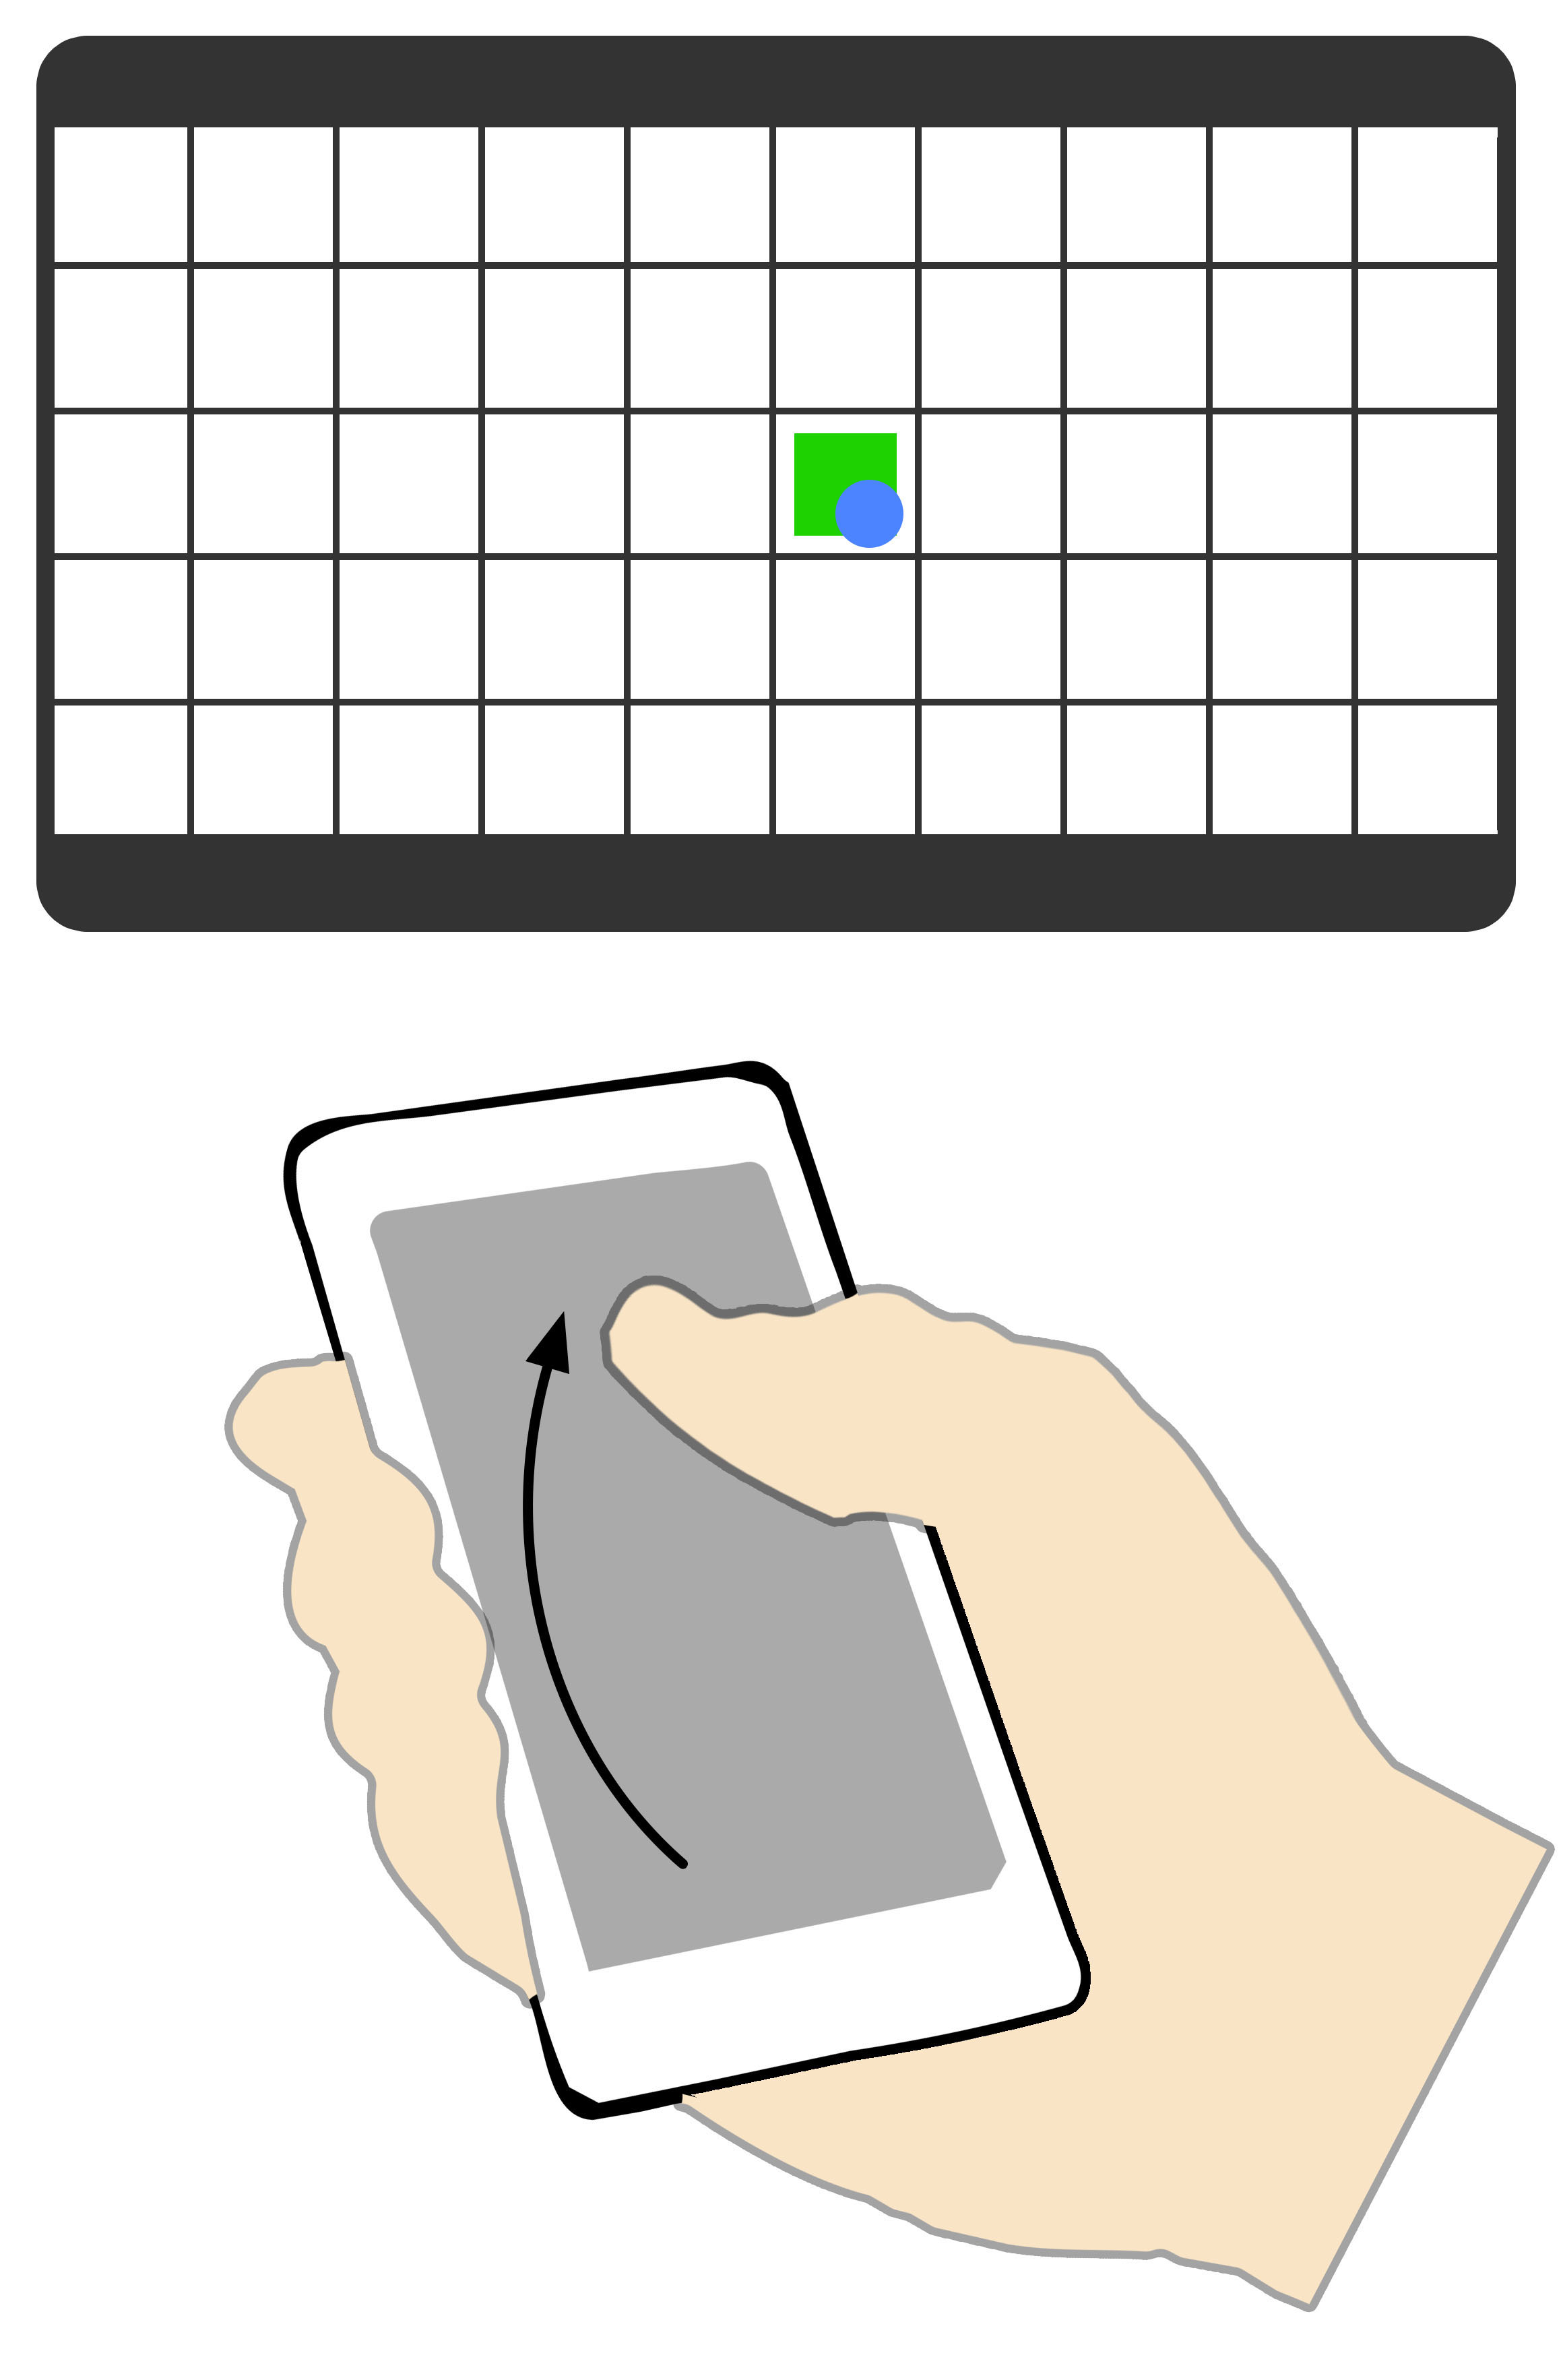
\includegraphics[width = 0.33\columnwidth]{images/techniques/swipePush3.jpg}\label{fig:swipePush3}}
	\caption{\push \grab technique}
	\label{fig:grabTechnique}
\end{figure}

\begin{figure}[H]
	\subfloat[]{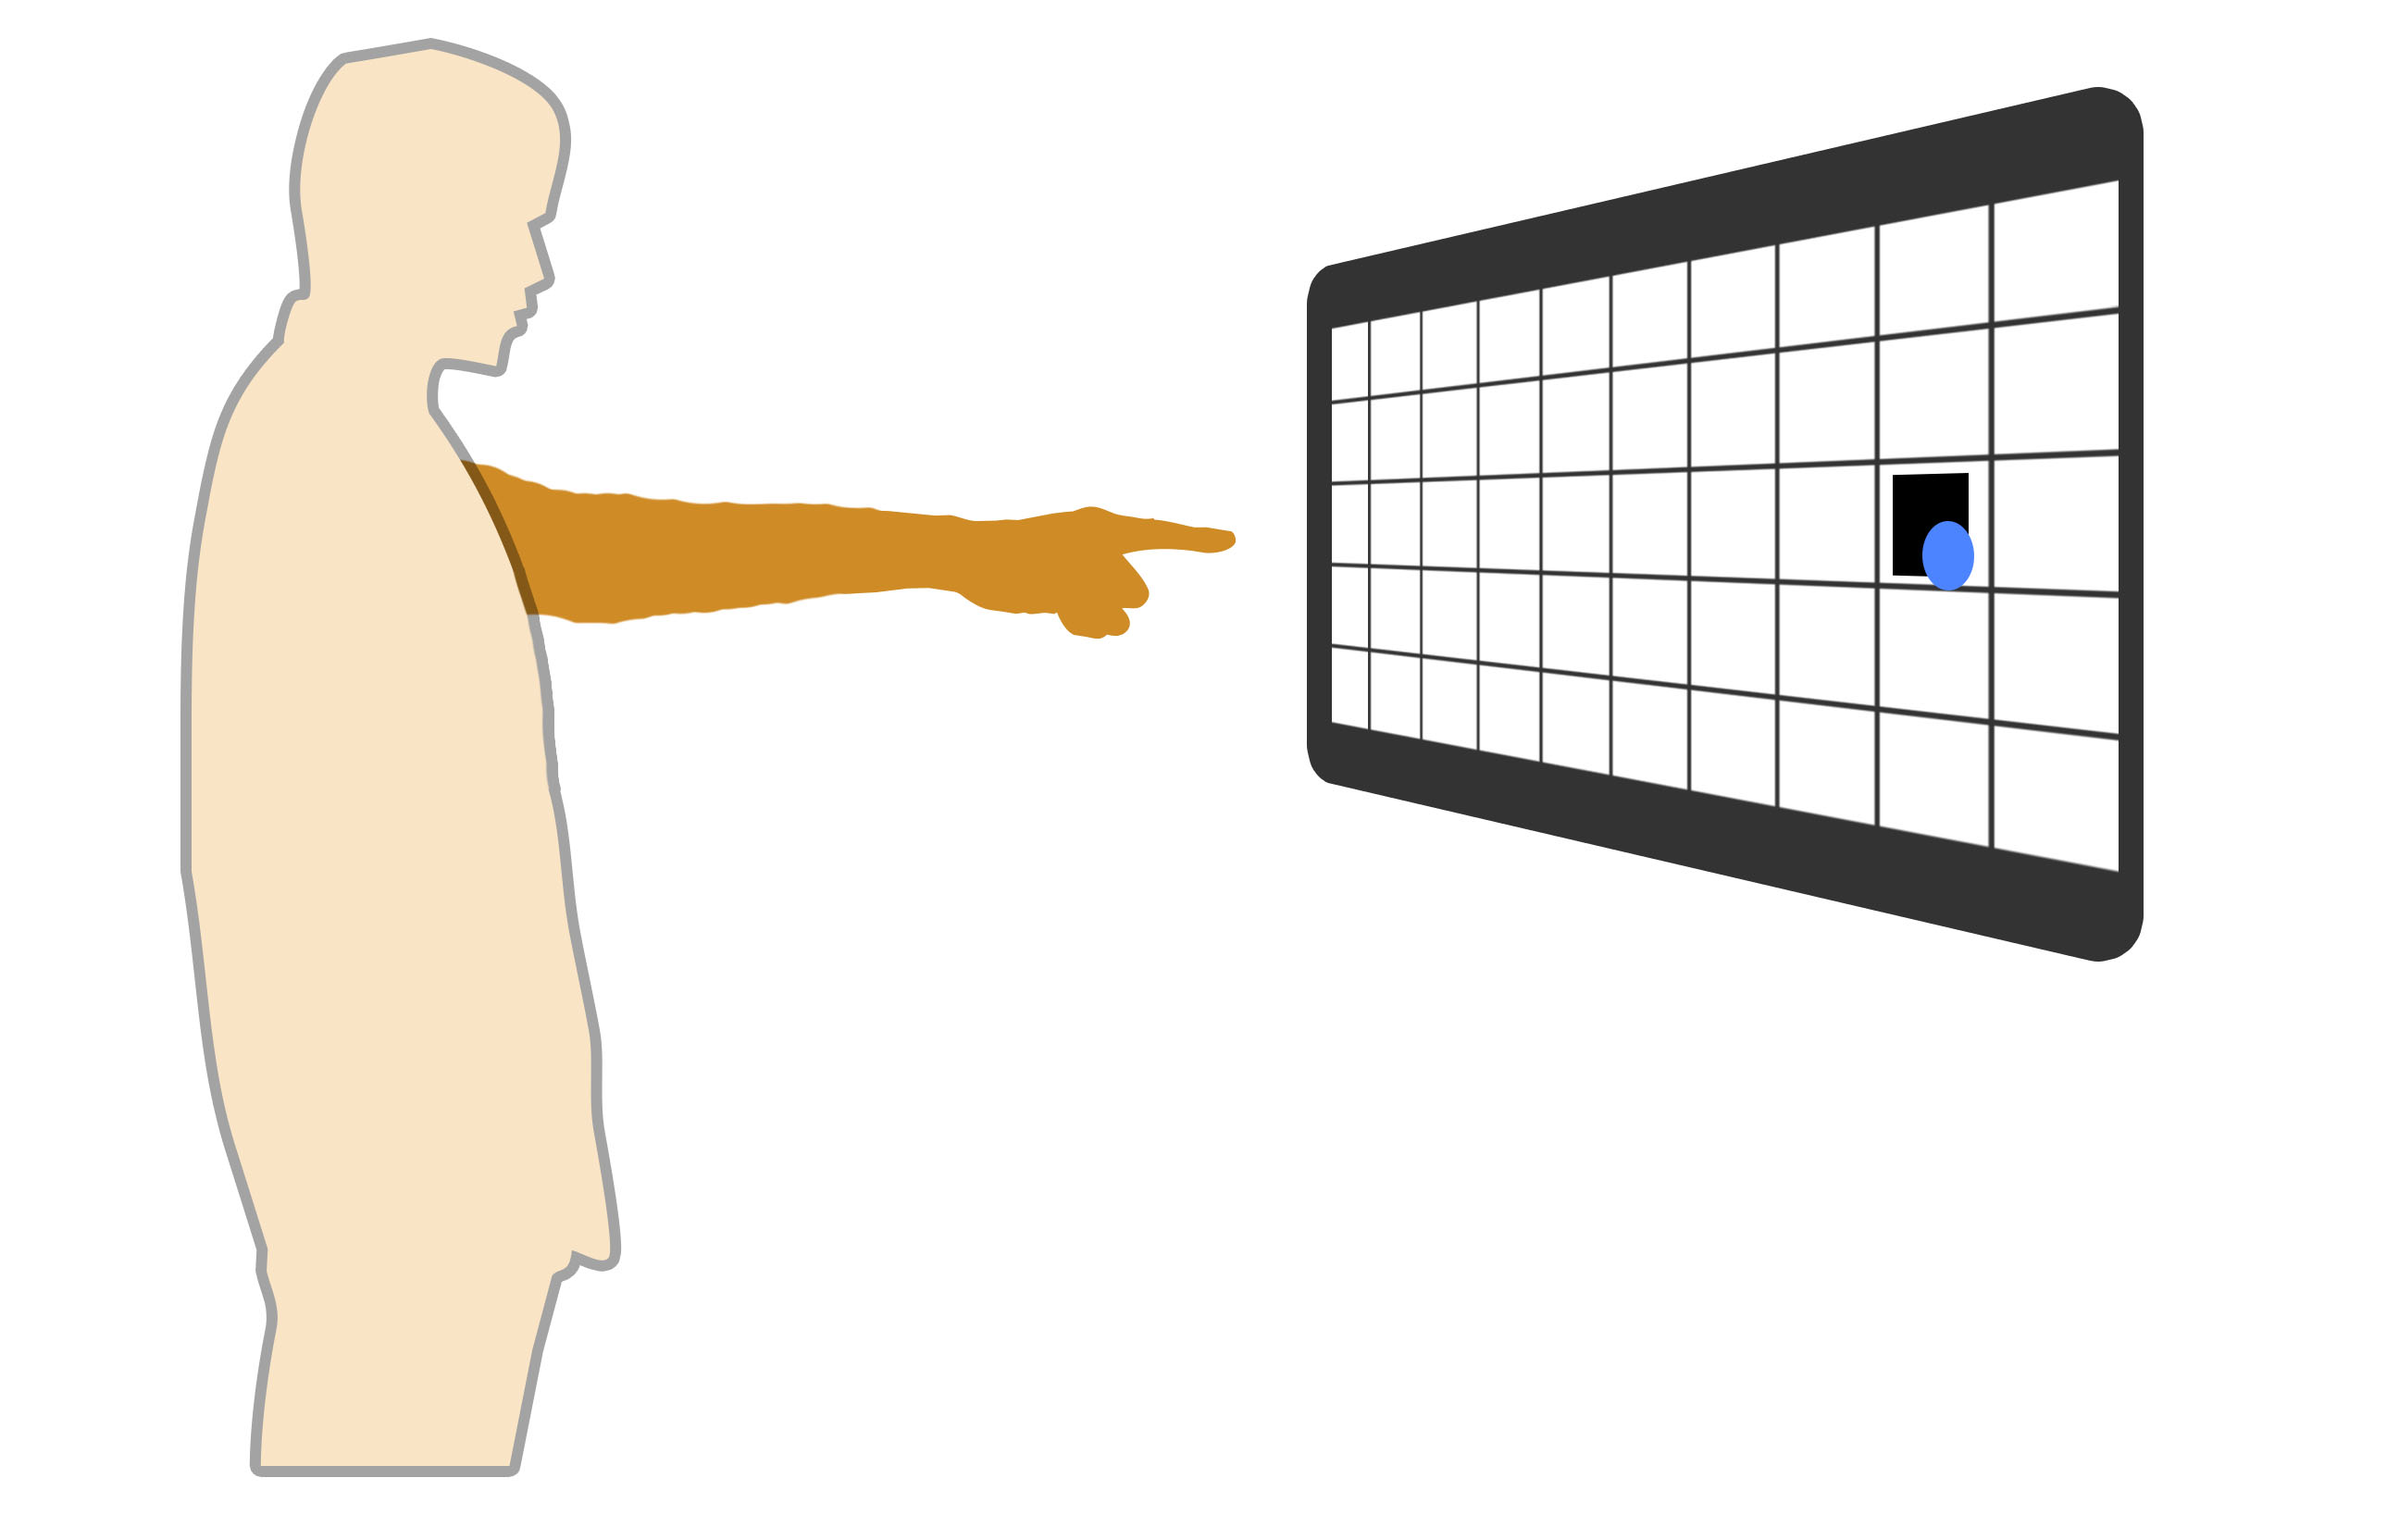
\includegraphics[width = 0.33\columnwidth]{images/techniques/throwPush1.jpg}\label{fig:throwPush1}}
	\subfloat[]{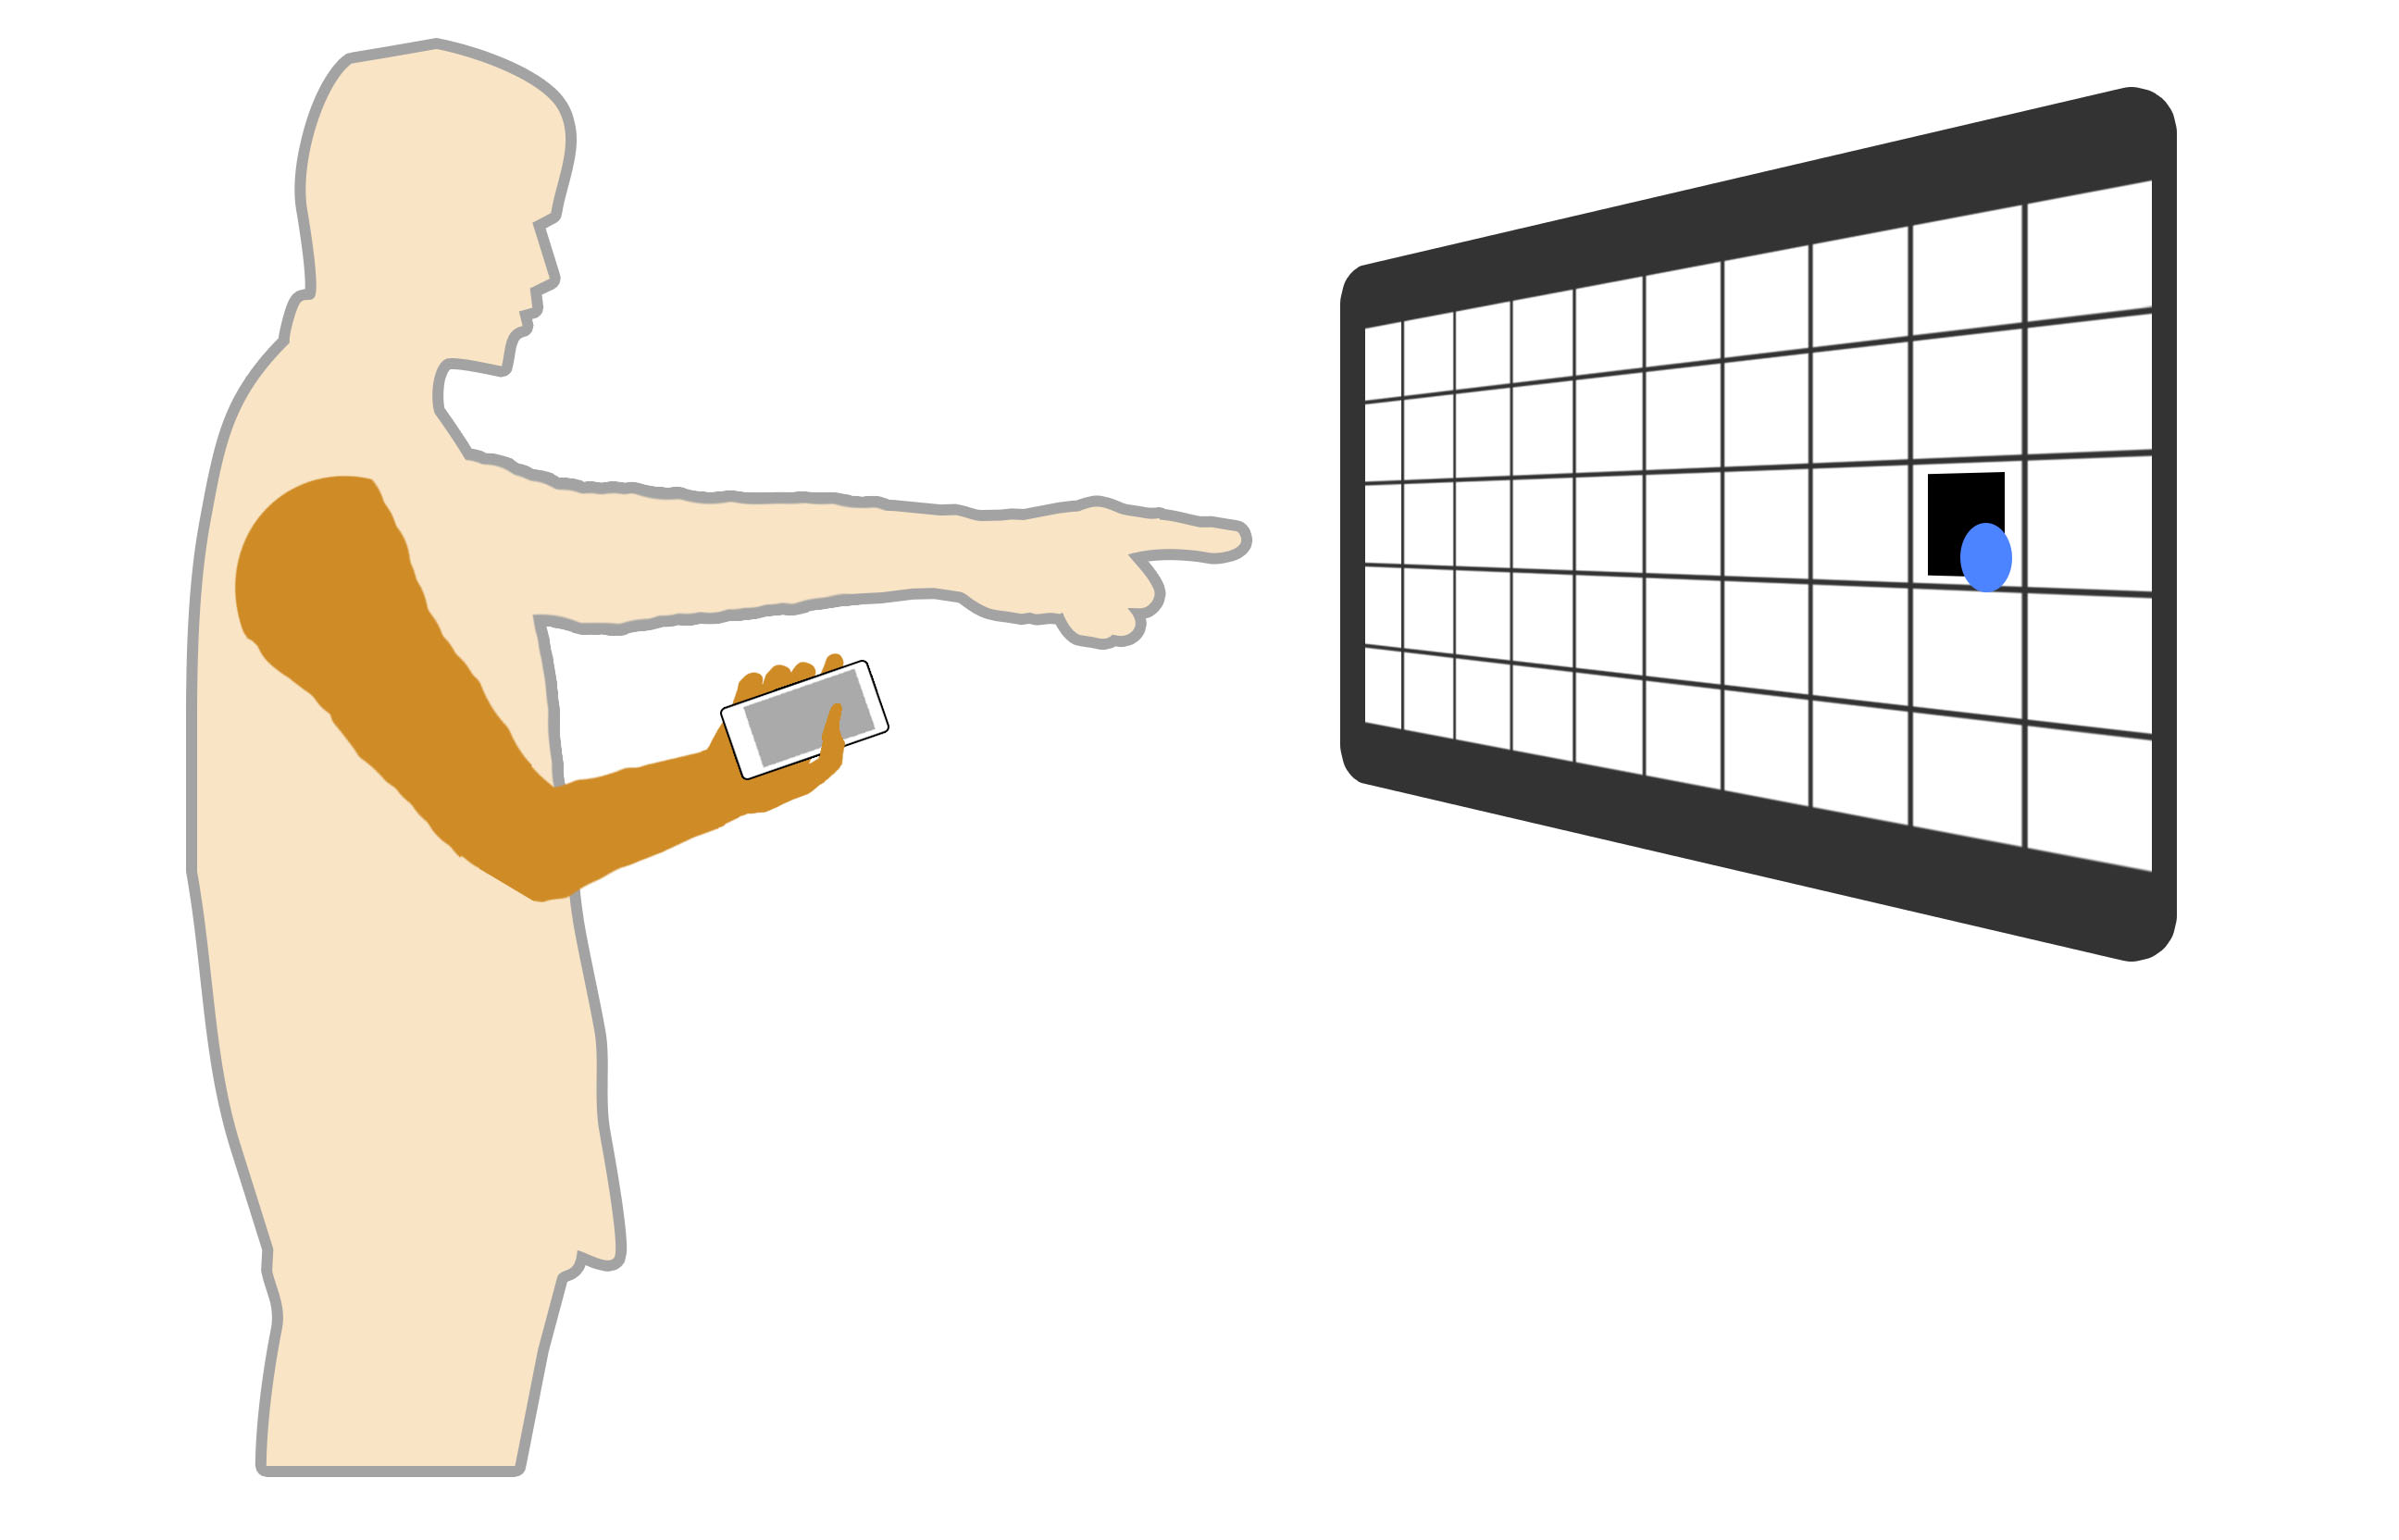
\includegraphics[width = 0.33\columnwidth]{images/techniques/throwPush2.jpg}\label{fig:throwPush2}}
	\subfloat[]{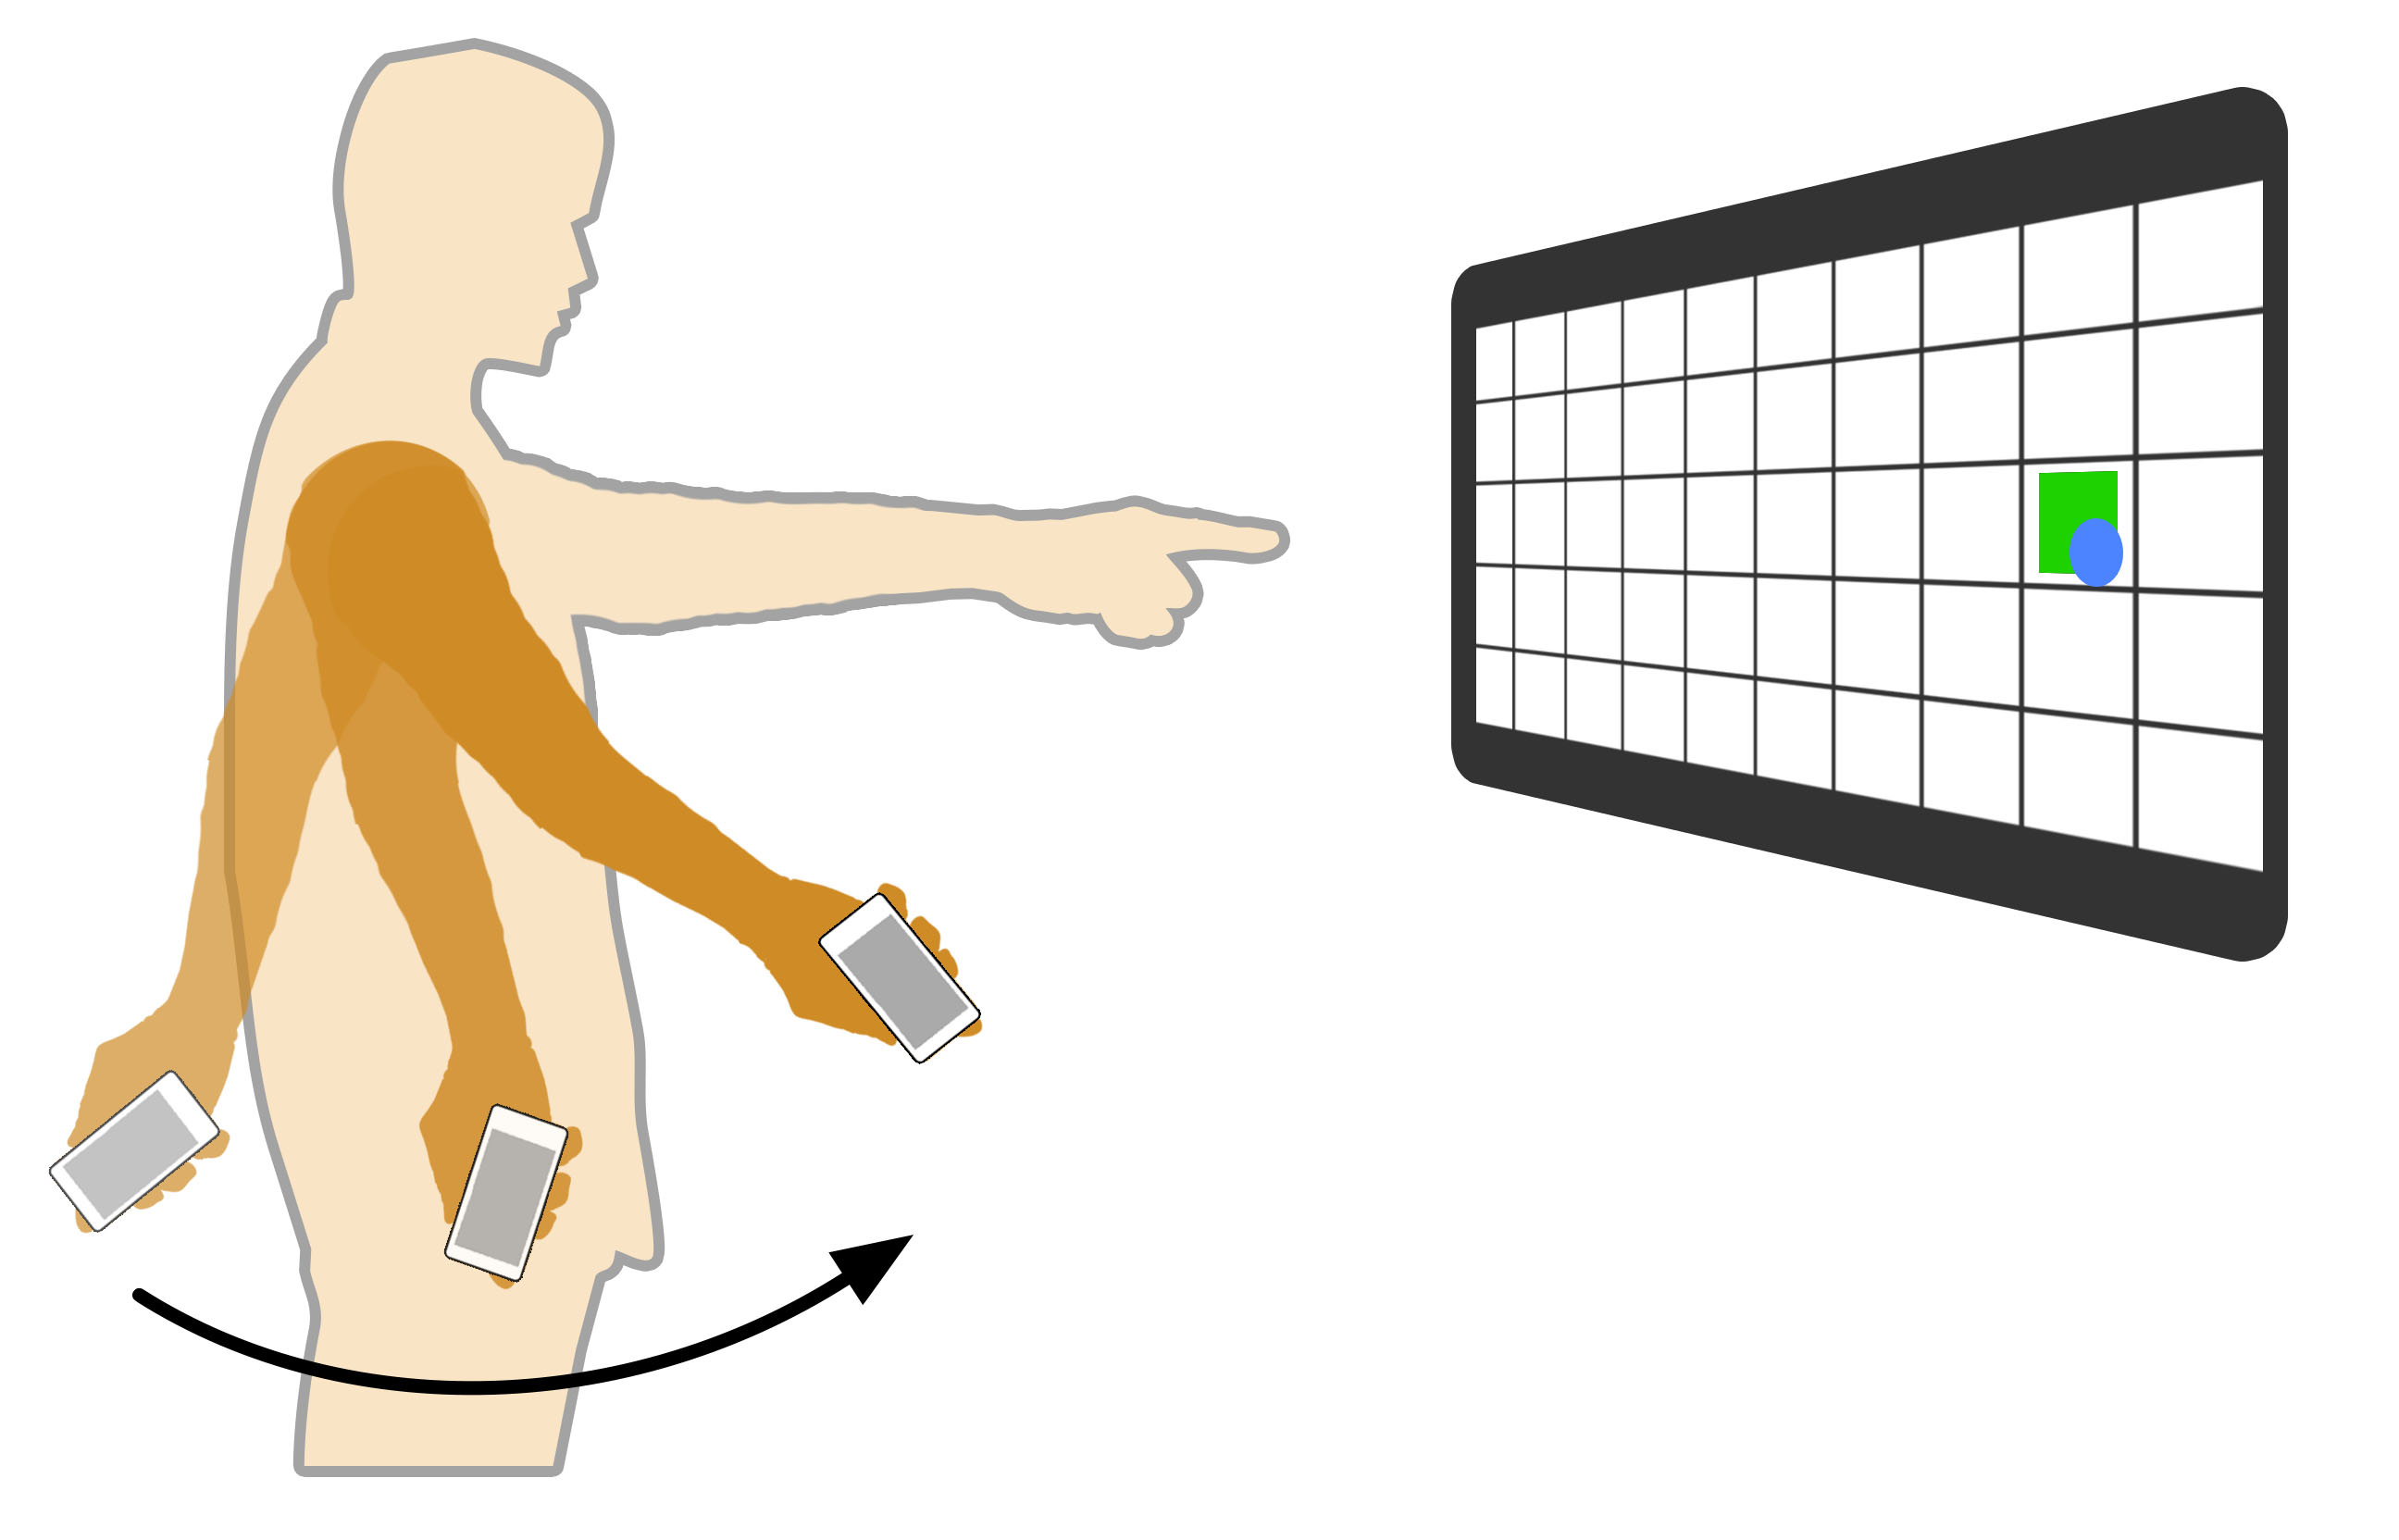
\includegraphics[width = 0.33\columnwidth]{images/techniques/throwPush3.jpg}\label{fig:throwPush3}}
	\caption{\push \grab technique}
	\label{fig:grabTechnique}
\end{figure}

\begin{figure}[H]
	\subfloat[]{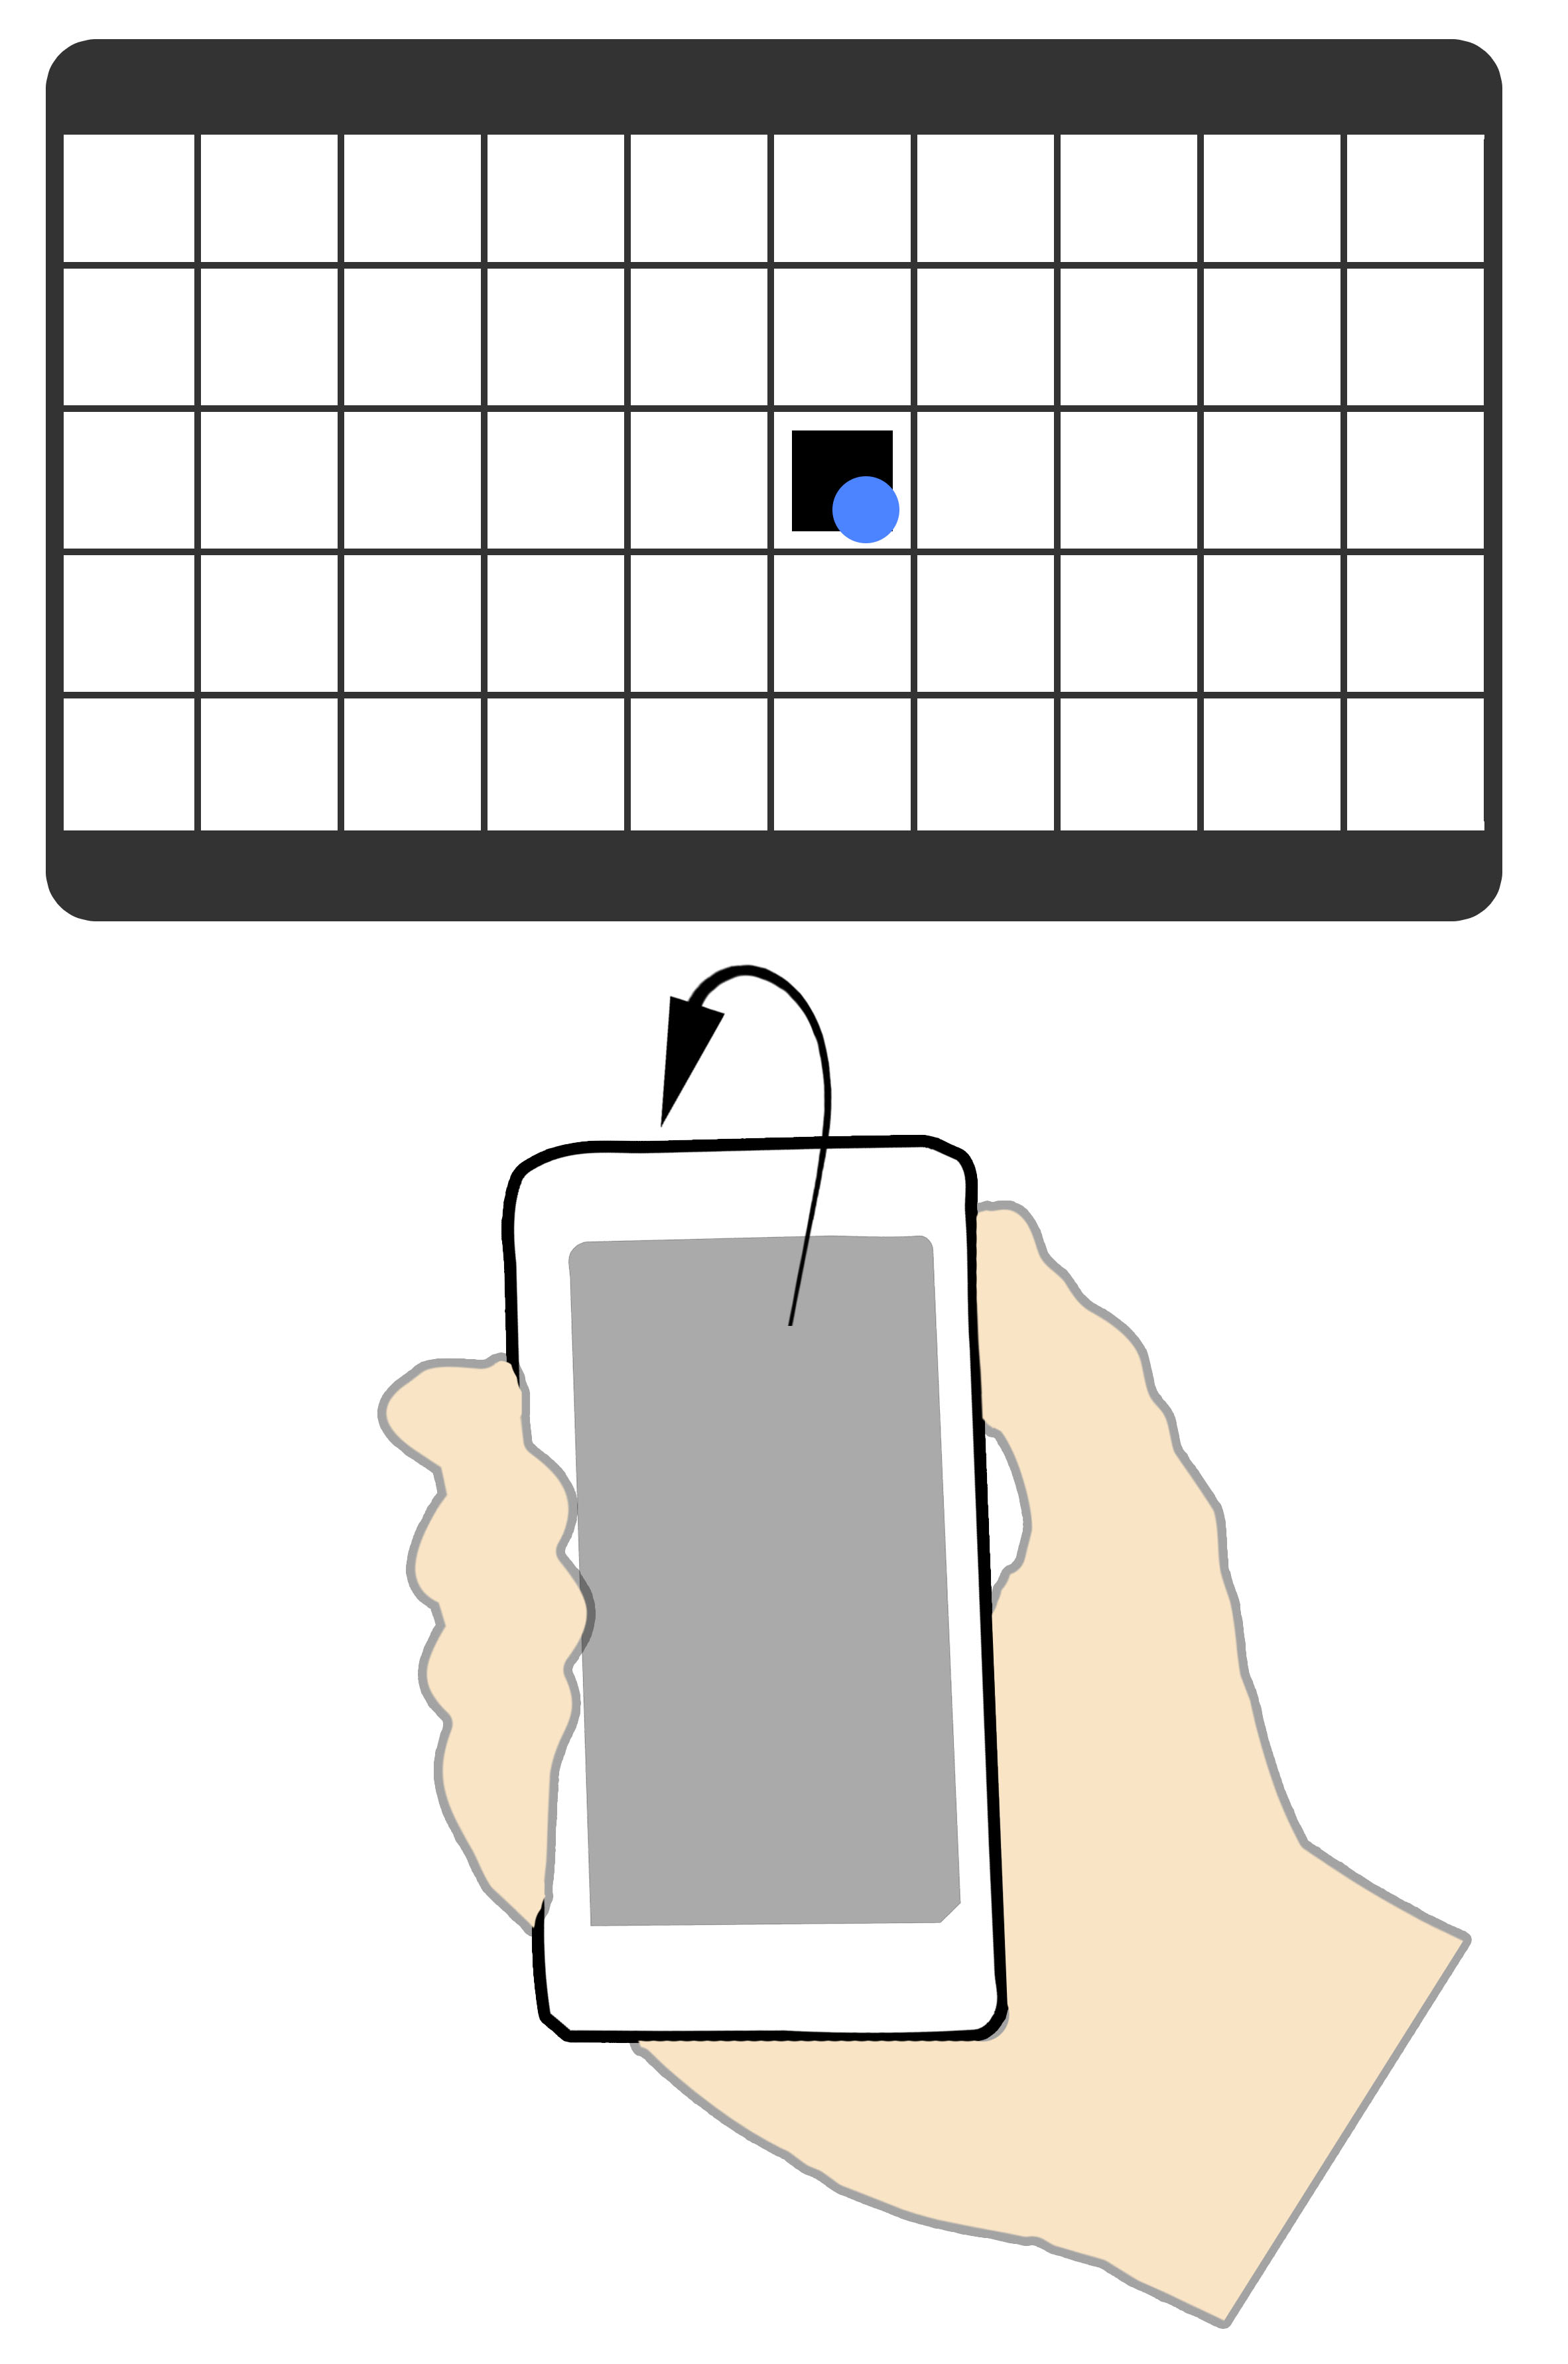
\includegraphics[width = 0.33\columnwidth]{images/techniques/tiltPush1.jpg}\label{fig:tiltPush1}}
	\subfloat[]{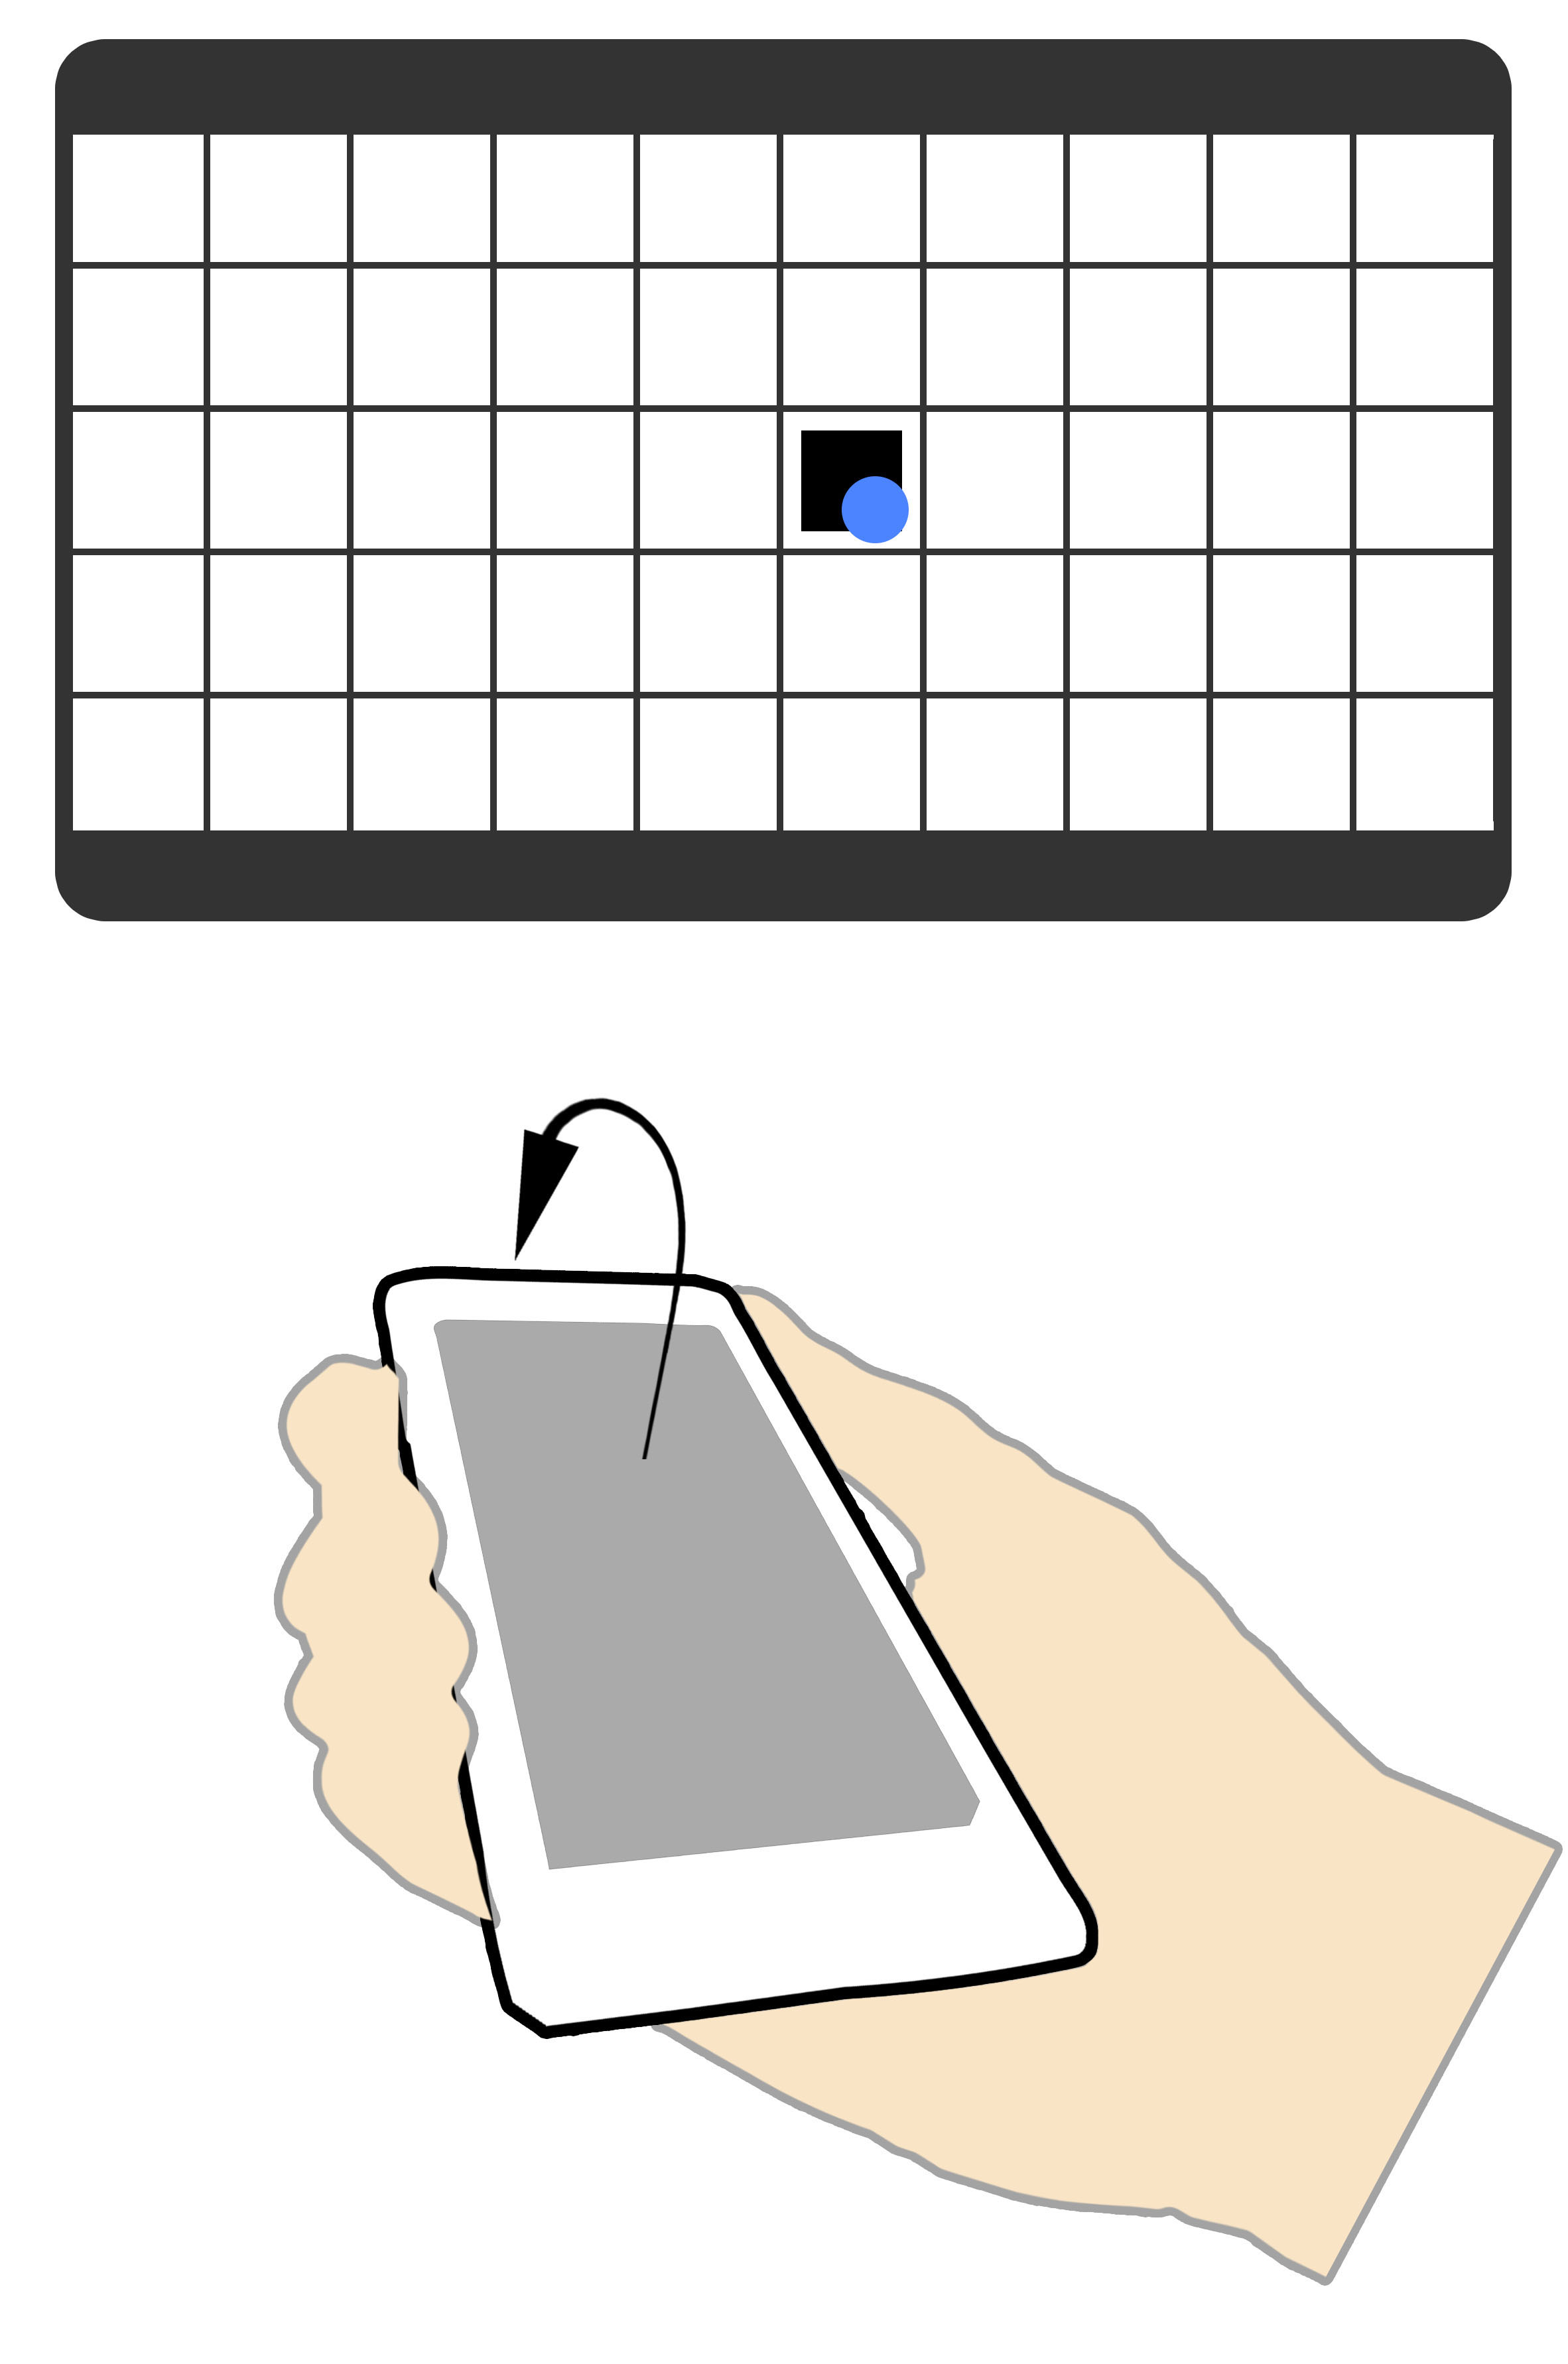
\includegraphics[width = 0.33\columnwidth]{images/techniques/tiltPush2.jpg}\label{fig:tiltPush2}}
	\subfloat[]{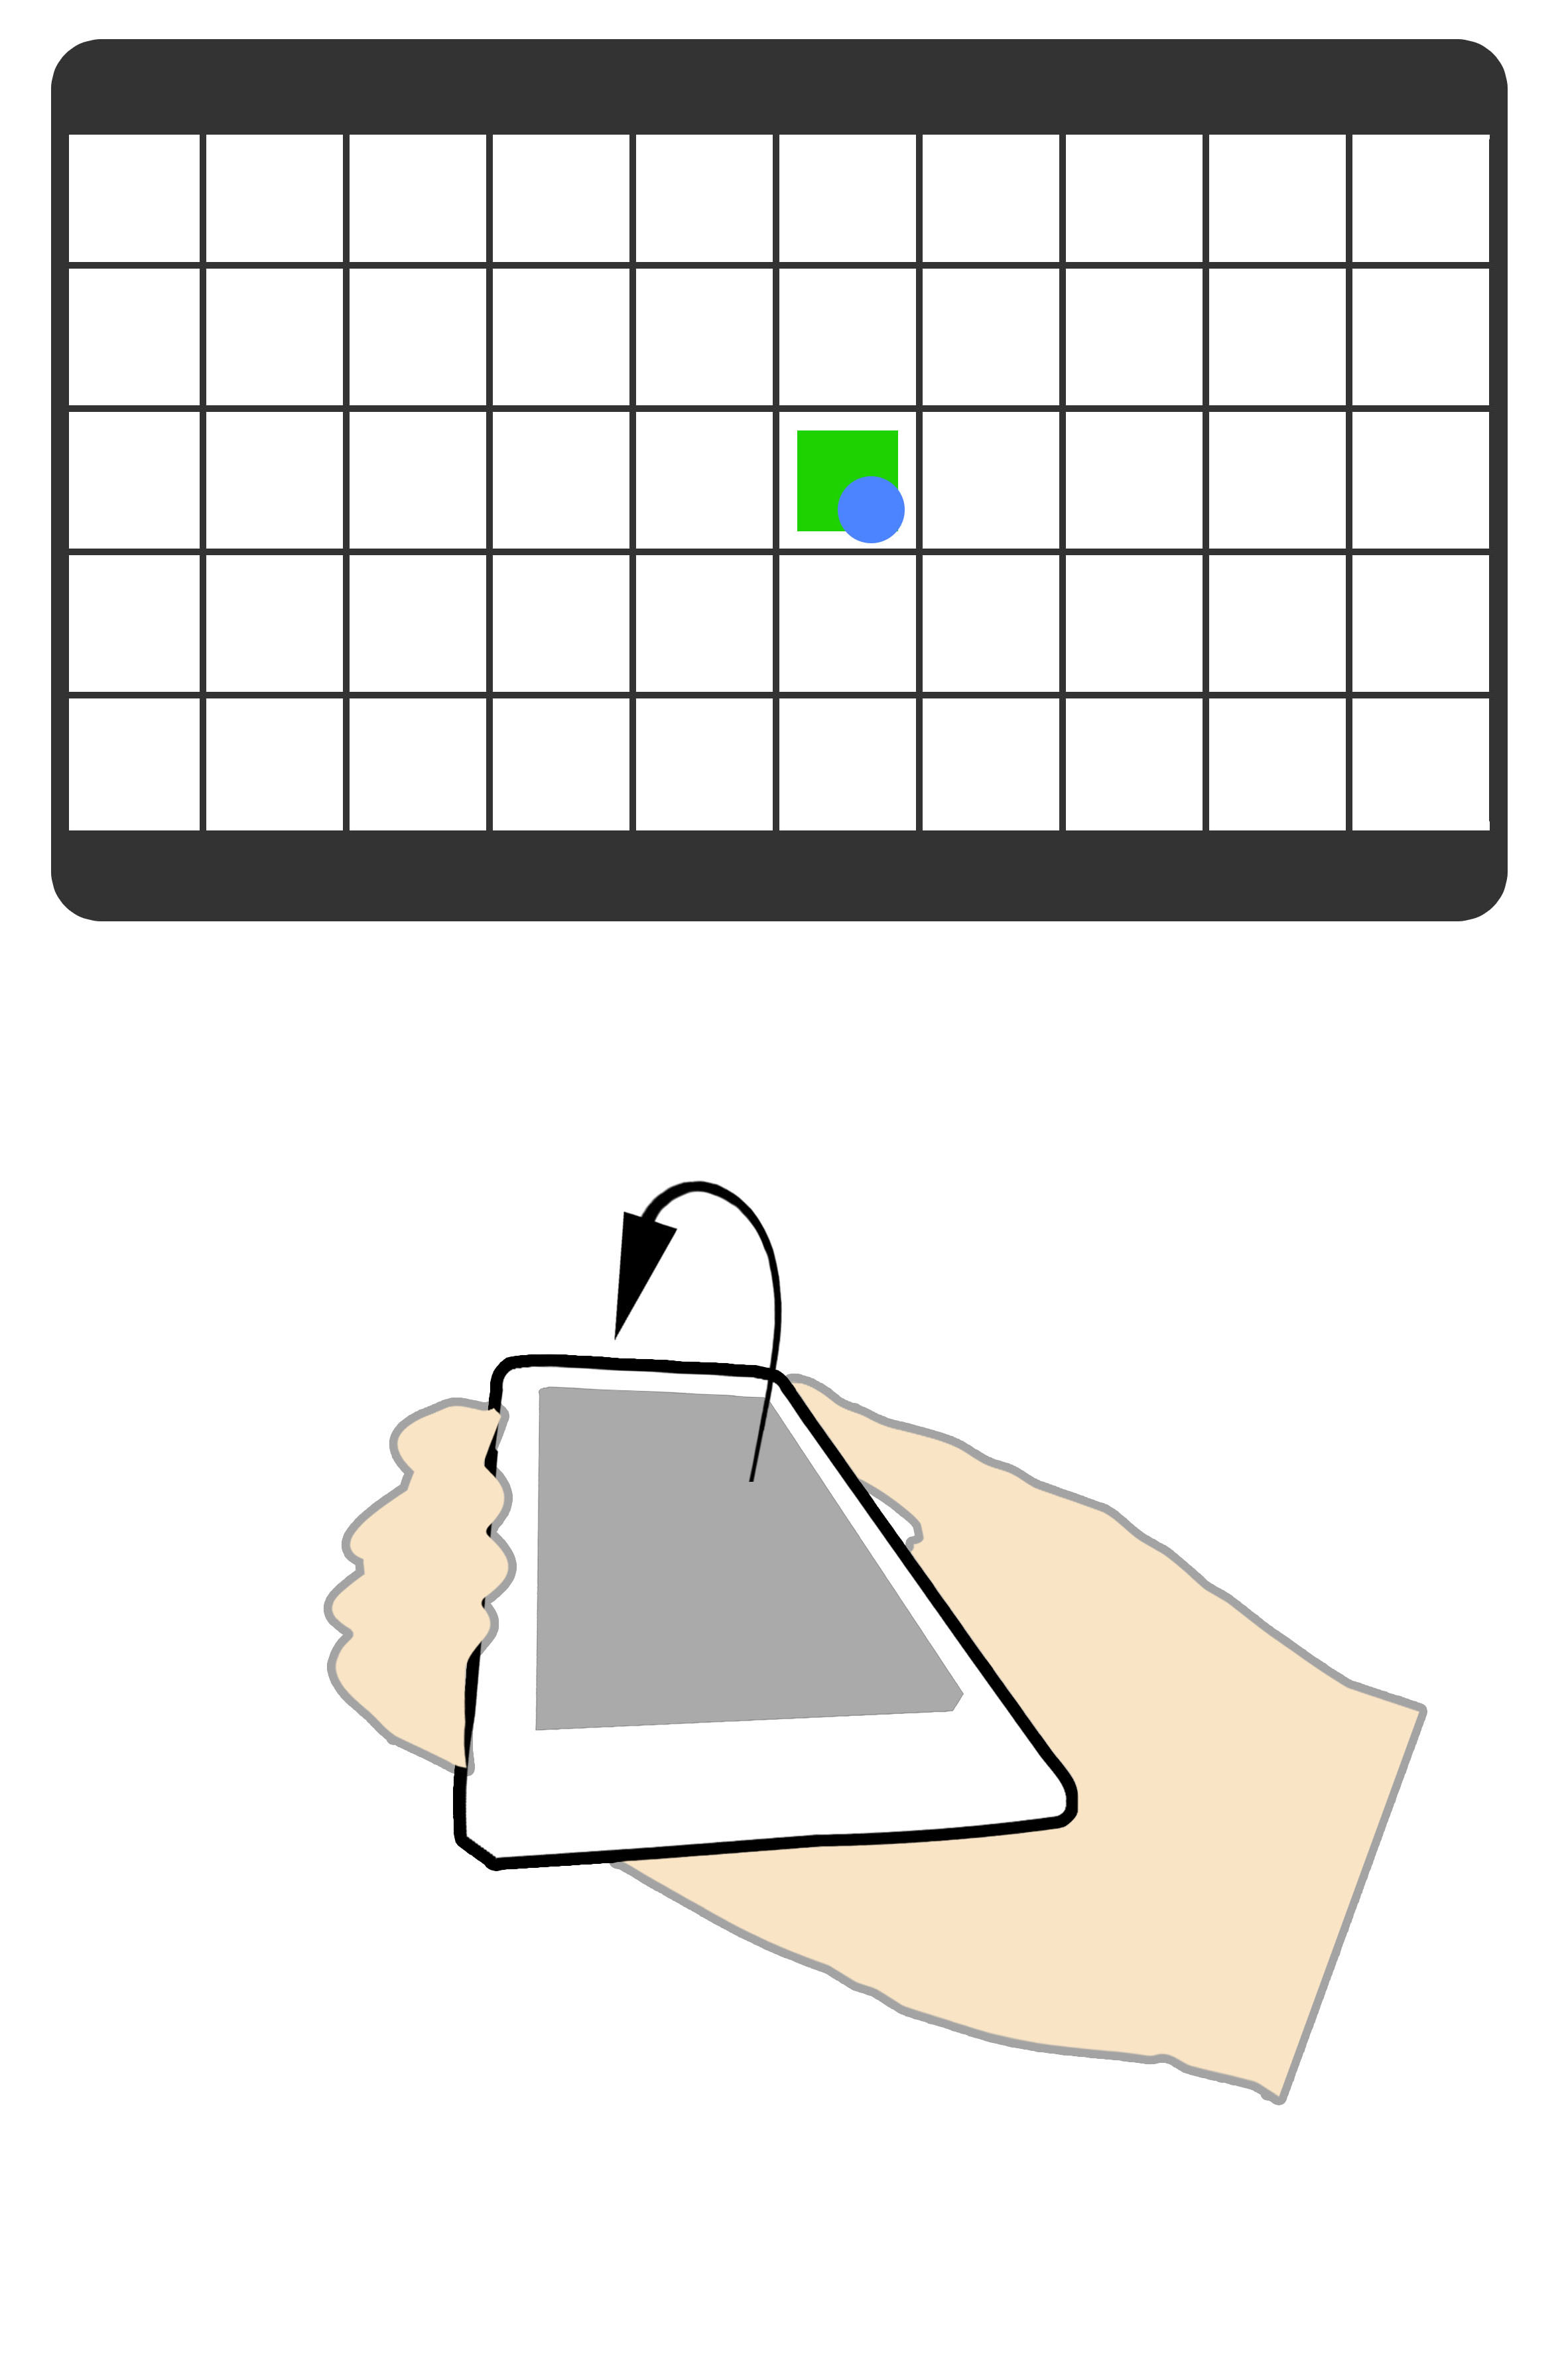
\includegraphics[width = 0.33\columnwidth]{images/techniques/tiltPush3.jpg}\label{fig:tiltPush3}}
	\caption{\push \grab technique}
	\label{fig:grabTechnique}
\end{figure}